% Options for packages loaded elsewhere
\PassOptionsToPackage{unicode}{hyperref}
\PassOptionsToPackage{hyphens}{url}
%
\documentclass[
]{article}
\title{MTH 3270 Notes 5}
\author{Tobias Boggess}
\date{2/28/2022}

\usepackage{amsmath,amssymb}
\usepackage{lmodern}
\usepackage{iftex}
\ifPDFTeX
  \usepackage[T1]{fontenc}
  \usepackage[utf8]{inputenc}
  \usepackage{textcomp} % provide euro and other symbols
\else % if luatex or xetex
  \usepackage{unicode-math}
  \defaultfontfeatures{Scale=MatchLowercase}
  \defaultfontfeatures[\rmfamily]{Ligatures=TeX,Scale=1}
\fi
% Use upquote if available, for straight quotes in verbatim environments
\IfFileExists{upquote.sty}{\usepackage{upquote}}{}
\IfFileExists{microtype.sty}{% use microtype if available
  \usepackage[]{microtype}
  \UseMicrotypeSet[protrusion]{basicmath} % disable protrusion for tt fonts
}{}
\makeatletter
\@ifundefined{KOMAClassName}{% if non-KOMA class
  \IfFileExists{parskip.sty}{%
    \usepackage{parskip}
  }{% else
    \setlength{\parindent}{0pt}
    \setlength{\parskip}{6pt plus 2pt minus 1pt}}
}{% if KOMA class
  \KOMAoptions{parskip=half}}
\makeatother
\usepackage{xcolor}
\IfFileExists{xurl.sty}{\usepackage{xurl}}{} % add URL line breaks if available
\IfFileExists{bookmark.sty}{\usepackage{bookmark}}{\usepackage{hyperref}}
\hypersetup{
  pdftitle={MTH 3270 Notes 5},
  pdfauthor={Tobias Boggess},
  hidelinks,
  pdfcreator={LaTeX via pandoc}}
\urlstyle{same} % disable monospaced font for URLs
\usepackage[margin=1in]{geometry}
\usepackage{color}
\usepackage{fancyvrb}
\newcommand{\VerbBar}{|}
\newcommand{\VERB}{\Verb[commandchars=\\\{\}]}
\DefineVerbatimEnvironment{Highlighting}{Verbatim}{commandchars=\\\{\}}
% Add ',fontsize=\small' for more characters per line
\usepackage{framed}
\definecolor{shadecolor}{RGB}{248,248,248}
\newenvironment{Shaded}{\begin{snugshade}}{\end{snugshade}}
\newcommand{\AlertTok}[1]{\textcolor[rgb]{0.94,0.16,0.16}{#1}}
\newcommand{\AnnotationTok}[1]{\textcolor[rgb]{0.56,0.35,0.01}{\textbf{\textit{#1}}}}
\newcommand{\AttributeTok}[1]{\textcolor[rgb]{0.77,0.63,0.00}{#1}}
\newcommand{\BaseNTok}[1]{\textcolor[rgb]{0.00,0.00,0.81}{#1}}
\newcommand{\BuiltInTok}[1]{#1}
\newcommand{\CharTok}[1]{\textcolor[rgb]{0.31,0.60,0.02}{#1}}
\newcommand{\CommentTok}[1]{\textcolor[rgb]{0.56,0.35,0.01}{\textit{#1}}}
\newcommand{\CommentVarTok}[1]{\textcolor[rgb]{0.56,0.35,0.01}{\textbf{\textit{#1}}}}
\newcommand{\ConstantTok}[1]{\textcolor[rgb]{0.00,0.00,0.00}{#1}}
\newcommand{\ControlFlowTok}[1]{\textcolor[rgb]{0.13,0.29,0.53}{\textbf{#1}}}
\newcommand{\DataTypeTok}[1]{\textcolor[rgb]{0.13,0.29,0.53}{#1}}
\newcommand{\DecValTok}[1]{\textcolor[rgb]{0.00,0.00,0.81}{#1}}
\newcommand{\DocumentationTok}[1]{\textcolor[rgb]{0.56,0.35,0.01}{\textbf{\textit{#1}}}}
\newcommand{\ErrorTok}[1]{\textcolor[rgb]{0.64,0.00,0.00}{\textbf{#1}}}
\newcommand{\ExtensionTok}[1]{#1}
\newcommand{\FloatTok}[1]{\textcolor[rgb]{0.00,0.00,0.81}{#1}}
\newcommand{\FunctionTok}[1]{\textcolor[rgb]{0.00,0.00,0.00}{#1}}
\newcommand{\ImportTok}[1]{#1}
\newcommand{\InformationTok}[1]{\textcolor[rgb]{0.56,0.35,0.01}{\textbf{\textit{#1}}}}
\newcommand{\KeywordTok}[1]{\textcolor[rgb]{0.13,0.29,0.53}{\textbf{#1}}}
\newcommand{\NormalTok}[1]{#1}
\newcommand{\OperatorTok}[1]{\textcolor[rgb]{0.81,0.36,0.00}{\textbf{#1}}}
\newcommand{\OtherTok}[1]{\textcolor[rgb]{0.56,0.35,0.01}{#1}}
\newcommand{\PreprocessorTok}[1]{\textcolor[rgb]{0.56,0.35,0.01}{\textit{#1}}}
\newcommand{\RegionMarkerTok}[1]{#1}
\newcommand{\SpecialCharTok}[1]{\textcolor[rgb]{0.00,0.00,0.00}{#1}}
\newcommand{\SpecialStringTok}[1]{\textcolor[rgb]{0.31,0.60,0.02}{#1}}
\newcommand{\StringTok}[1]{\textcolor[rgb]{0.31,0.60,0.02}{#1}}
\newcommand{\VariableTok}[1]{\textcolor[rgb]{0.00,0.00,0.00}{#1}}
\newcommand{\VerbatimStringTok}[1]{\textcolor[rgb]{0.31,0.60,0.02}{#1}}
\newcommand{\WarningTok}[1]{\textcolor[rgb]{0.56,0.35,0.01}{\textbf{\textit{#1}}}}
\usepackage{graphicx}
\makeatletter
\def\maxwidth{\ifdim\Gin@nat@width>\linewidth\linewidth\else\Gin@nat@width\fi}
\def\maxheight{\ifdim\Gin@nat@height>\textheight\textheight\else\Gin@nat@height\fi}
\makeatother
% Scale images if necessary, so that they will not overflow the page
% margins by default, and it is still possible to overwrite the defaults
% using explicit options in \includegraphics[width, height, ...]{}
\setkeys{Gin}{width=\maxwidth,height=\maxheight,keepaspectratio}
% Set default figure placement to htbp
\makeatletter
\def\fps@figure{htbp}
\makeatother
\setlength{\emergencystretch}{3em} % prevent overfull lines
\providecommand{\tightlist}{%
  \setlength{\itemsep}{0pt}\setlength{\parskip}{0pt}}
\setcounter{secnumdepth}{-\maxdimen} % remove section numbering
\ifLuaTeX
  \usepackage{selnolig}  % disable illegal ligatures
\fi

\begin{document}
\maketitle

\hypertarget{section-9.3-exercises}{%
\subsection{Section 9.3 Exercises}\label{section-9.3-exercises}}

\hypertarget{exercise-1-do-the-following.}{%
\subsubsection{Exercise 1: Do the
following.}\label{exercise-1-do-the-following.}}

\hypertarget{a-using-a-for-loop-and-rnorm-simulate-1000-random-samples-of-size-n-10-from-a-n50-15-population-i.e.-ux3bc-50-and-ux3c3-15-compute-the-sample-mean-x-of-each-sample-and-store-the-x-values-in-a-1000-element-vector-named-say-sim.sample_means.-report-your-r-commands.}{%
\paragraph{a) Using a for() loop and rnorm(), simulate 1,000 random
samples of size n = 10 from a N(50, 15) population (i.e.~μ = 50 and σ =
15), compute the sample mean ̄X of each sample, and store the ̄X values
in a 1,000-element vector named, say, sim.sample\_means. Report your R
command(s).}\label{a-using-a-for-loop-and-rnorm-simulate-1000-random-samples-of-size-n-10-from-a-n50-15-population-i.e.-ux3bc-50-and-ux3c3-15-compute-the-sample-mean-x-of-each-sample-and-store-the-x-values-in-a-1000-element-vector-named-say-sim.sample_means.-report-your-r-commands.}}

Code:

\begin{Shaded}
\begin{Highlighting}[]
\NormalTok{sim.sample\_means }\OtherTok{\textless{}{-}} \FunctionTok{rep}\NormalTok{(}\ConstantTok{NA}\NormalTok{, }\DecValTok{1000}\NormalTok{)}
\ControlFlowTok{for}\NormalTok{(i }\ControlFlowTok{in} \DecValTok{1}\SpecialCharTok{:}\DecValTok{1000}\NormalTok{) \{}
\NormalTok{  sim.sample }\OtherTok{\textless{}{-}} \FunctionTok{rnorm}\NormalTok{(}\AttributeTok{n =} \DecValTok{10}\NormalTok{, }\AttributeTok{mean =} \DecValTok{50}\NormalTok{, }\AttributeTok{sd =} \DecValTok{15}\NormalTok{)}
\NormalTok{  sim.sample\_means[i] }\OtherTok{\textless{}{-}} \FunctionTok{mean}\NormalTok{(sim.sample)}
\NormalTok{\}}
\FunctionTok{head}\NormalTok{(sim.sample\_means, }\DecValTok{5}\NormalTok{)}
\end{Highlighting}
\end{Shaded}

\begin{verbatim}
## [1] 48.84105 51.49588 43.95355 53.74380 55.76600
\end{verbatim}

\hypertarget{b-now-use-mean-and-sd-to-compute-the-mean-and-standard-error-of-the-1000-x-values.-report-these-two-values.}{%
\paragraph{b) Now use mean() and sd() to compute the mean and standard
error of the 1,000 ̄X values. Report these two
values.}\label{b-now-use-mean-and-sd-to-compute-the-mean-and-standard-error-of-the-1000-x-values.-report-these-two-values.}}

Code:

\begin{Shaded}
\begin{Highlighting}[]
\NormalTok{sim.mean }\OtherTok{\textless{}{-}} \FunctionTok{mean}\NormalTok{(sim.sample\_means)}
\NormalTok{sim.mean}
\end{Highlighting}
\end{Shaded}

\begin{verbatim}
## [1] 49.95189
\end{verbatim}

\begin{Shaded}
\begin{Highlighting}[]
\NormalTok{sim.sd }\OtherTok{\textless{}{-}} \FunctionTok{sd}\NormalTok{(sim.sample\_means)}
\NormalTok{sim.sd}
\end{Highlighting}
\end{Shaded}

\begin{verbatim}
## [1] 4.638603
\end{verbatim}

\newpage

\hypertarget{c-recall-that-if-a-random-sample-of-size-n-is-drawn-from-a-nux3bc-ux3c3-population-the-sampling-distribution-of-x-obtained-via-mathematical-theory-is-nux3bc-ux3c3n.compare-the-two-values-of-part-a-to-the-theoretical-mean-and-standard-error-ux3bc-and-ux3c3n-of-the-sampling-distribution-of-x.}{%
\paragraph{c) Recall that if a random sample of size n is drawn from a
N(μ, σ) population, the sampling distribution of ̄X (obtained via
mathematical theory) is N(μ, σ/√n).Compare the two values of Part a to
the theoretical mean and standard error, μ and σ/√n, of the sampling
distribution of
̄X.}\label{c-recall-that-if-a-random-sample-of-size-n-is-drawn-from-a-nux3bc-ux3c3-population-the-sampling-distribution-of-x-obtained-via-mathematical-theory-is-nux3bc-ux3c3n.compare-the-two-values-of-part-a-to-the-theoretical-mean-and-standard-error-ux3bc-and-ux3c3n-of-the-sampling-distribution-of-x.}}

Code:

\begin{Shaded}
\begin{Highlighting}[]
\NormalTok{diff.x\_bar }\OtherTok{\textless{}{-}}\NormalTok{ sim.mean }\SpecialCharTok{{-}} \DecValTok{50}
\NormalTok{diff.x\_bar}
\end{Highlighting}
\end{Shaded}

\begin{verbatim}
## [1] -0.04810946
\end{verbatim}

\begin{Shaded}
\begin{Highlighting}[]
\NormalTok{diff.x\_sd }\OtherTok{\textless{}{-}}\NormalTok{ sim.sd }\SpecialCharTok{{-}}\NormalTok{ (}\DecValTok{15} \SpecialCharTok{/} \FunctionTok{sqrt}\NormalTok{(}\DecValTok{1000}\NormalTok{))}
\NormalTok{diff.x\_sd}
\end{Highlighting}
\end{Shaded}

\begin{verbatim}
## [1] 4.164261
\end{verbatim}

\newpage

\hypertarget{d-make-a-histogram-of-the-1000-simulated-x-values.-compare-the-shape-center-and-spread-of-the-histogram-to-the-theoretical-nux3bc-ux3c3n-sampling-distribution-of-x.}{%
\paragraph{d) Make a histogram of the 1,000 simulated ̄X values. Compare
the shape, center, and spread of the histogram to the theoretical N(μ,
σ/√n) sampling distribution of
̄X.}\label{d-make-a-histogram-of-the-1000-simulated-x-values.-compare-the-shape-center-and-spread-of-the-histogram-to-the-theoretical-nux3bc-ux3c3n-sampling-distribution-of-x.}}

Code:

\begin{Shaded}
\begin{Highlighting}[]
\FunctionTok{library}\NormalTok{(ggplot2)}

\FunctionTok{ggplot}\NormalTok{(}\AttributeTok{data =} \FunctionTok{data.frame}\NormalTok{(sim.sample\_means)) }\SpecialCharTok{+}
  \FunctionTok{geom\_histogram}\NormalTok{(}\AttributeTok{mapping =} \FunctionTok{aes}\NormalTok{(}\AttributeTok{x =}\NormalTok{ sim.sample\_means, }\AttributeTok{y =} \FunctionTok{stat}\NormalTok{(density))) }\SpecialCharTok{+}
  \FunctionTok{geom\_function}\NormalTok{(}\AttributeTok{fun =}\NormalTok{ dnorm,}
                \AttributeTok{args =} \FunctionTok{list}\NormalTok{(}\AttributeTok{mean =} \DecValTok{50}\NormalTok{, }\AttributeTok{sd =} \DecValTok{15} \SpecialCharTok{/} \FunctionTok{sqrt}\NormalTok{(}\DecValTok{10}\NormalTok{)),}
                \AttributeTok{color =} \StringTok{"blue"}\NormalTok{) }\SpecialCharTok{+}
  \FunctionTok{labs}\NormalTok{(}\AttributeTok{title =} \StringTok{"Sampling Distribution"}\NormalTok{)}
\end{Highlighting}
\end{Shaded}

\begin{verbatim}
## `stat_bin()` using `bins = 30`. Pick better value with `binwidth`.
\end{verbatim}

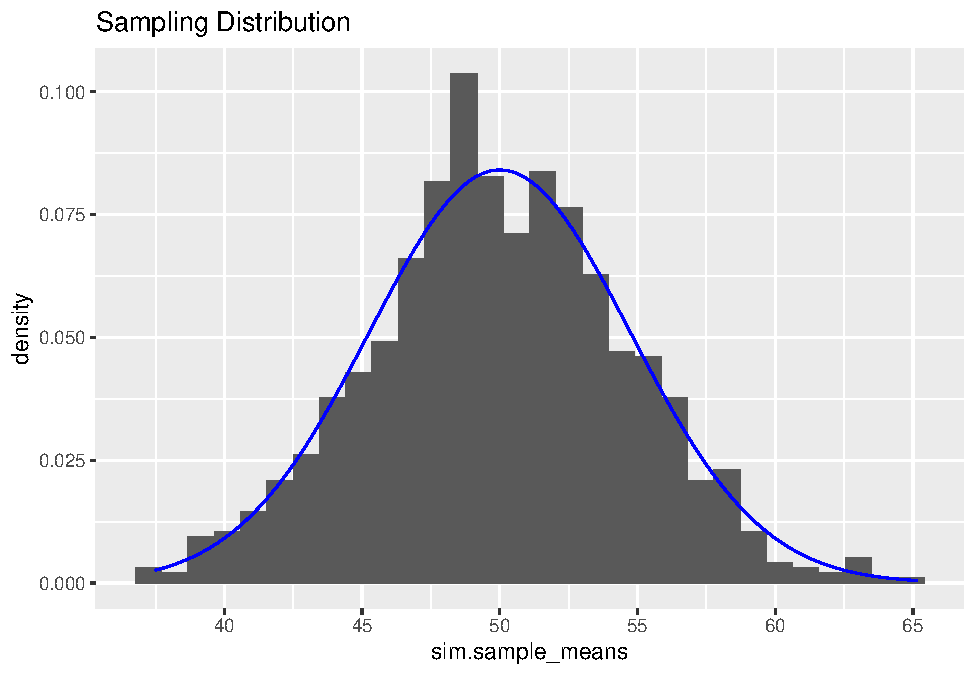
\includegraphics{Class_Exercises_ClassNotes_5_files/figure-latex/unnamed-chunk-4-1.pdf}
\newpage

\hypertarget{exercise-2-simulate-1000-random-samples-of-size-n-5-from-a-n50-15-population-i.e.-ux3bc-50-and-ux3c3-15-and-compute-the-four-statistics-below-for-each-sample.in-each-case-1-report-the-mean-and-standard-error-of-the-simulated-statistic-values-and-2-plot-the-simulated-values-in-a-histogram-and-describe-the-shape-center-and-spread-of-this-sampling-distribution.}{%
\subsubsection{Exercise 2: Simulate 1,000 random samples of size n = 5
from a N(50, 15) population (i.e.~μ = 50 and σ = 15), and compute the
four statistics below for each sample.In each case: 1) Report the mean
and standard error of the simulated statistic values, and 2) Plot the
simulated values in a histogram and describe the shape, center, and
spread of this sampling
distribution.}\label{exercise-2-simulate-1000-random-samples-of-size-n-5-from-a-n50-15-population-i.e.-ux3bc-50-and-ux3c3-15-and-compute-the-four-statistics-below-for-each-sample.in-each-case-1-report-the-mean-and-standard-error-of-the-simulated-statistic-values-and-2-plot-the-simulated-values-in-a-histogram-and-describe-the-shape-center-and-spread-of-this-sampling-distribution.}}

\hypertarget{a-the-sample-median-x-use-median.}{%
\paragraph{a) The sample median ̃X (use
median()).}\label{a-the-sample-median-x-use-median.}}

\hypertarget{b-the-sample-standard-deviation-s-use-sd.}{%
\paragraph{b) The sample standard deviation S (use
sd()).}\label{b-the-sample-standard-deviation-s-use-sd.}}

\hypertarget{c-the-sample-minimum-x1-use-min.}{%
\paragraph{c) The sample minimum X(1) (use
min()).}\label{c-the-sample-minimum-x1-use-min.}}

\hypertarget{d-the-sample-maximum-xn-use-max.}{%
\paragraph{d) The sample maximum X(n) (use
max()).}\label{d-the-sample-maximum-xn-use-max.}}

Code:

\begin{Shaded}
\begin{Highlighting}[]
\NormalTok{rand\_samp\_median }\OtherTok{\textless{}{-}} \FunctionTok{rep}\NormalTok{(}\ConstantTok{NA}\NormalTok{, }\DecValTok{1000}\NormalTok{)}
\NormalTok{rand\_samp\_min }\OtherTok{\textless{}{-}} \FunctionTok{rep}\NormalTok{(}\ConstantTok{NA}\NormalTok{, }\DecValTok{1000}\NormalTok{)}
\NormalTok{rand\_samp\_max }\OtherTok{\textless{}{-}} \FunctionTok{rep}\NormalTok{(}\ConstantTok{NA}\NormalTok{, }\DecValTok{1000}\NormalTok{)}
\NormalTok{rand\_samp\_sd }\OtherTok{\textless{}{-}} \FunctionTok{rep}\NormalTok{(}\ConstantTok{NA}\NormalTok{, }\DecValTok{1000}\NormalTok{)}

\ControlFlowTok{for}\NormalTok{ (i }\ControlFlowTok{in} \DecValTok{1}\SpecialCharTok{:}\DecValTok{1000}\NormalTok{) \{}
\NormalTok{  rand\_samp }\OtherTok{\textless{}{-}} \FunctionTok{rnorm}\NormalTok{(}\AttributeTok{n =} \DecValTok{5}\NormalTok{, }\AttributeTok{mean =} \DecValTok{50}\NormalTok{, }\AttributeTok{sd =} \DecValTok{15}\NormalTok{)}
\NormalTok{  rand\_samp\_median[i] }\OtherTok{\textless{}{-}} \FunctionTok{median}\NormalTok{(rand\_samp)}
\NormalTok{  rand\_samp\_sd[i] }\OtherTok{\textless{}{-}} \FunctionTok{sd}\NormalTok{(rand\_samp)}
\NormalTok{  rand\_samp\_min[i] }\OtherTok{\textless{}{-}} \FunctionTok{min}\NormalTok{(rand\_samp)}
\NormalTok{  rand\_samp\_max[i] }\OtherTok{\textless{}{-}} \FunctionTok{max}\NormalTok{(rand\_samp)}
\NormalTok{\}}

\NormalTok{mean.of\_median }\OtherTok{\textless{}{-}} \FunctionTok{mean}\NormalTok{(rand\_samp\_median)}
\NormalTok{mean.of\_sd }\OtherTok{\textless{}{-}} \FunctionTok{mean}\NormalTok{(rand\_samp\_sd)}
\NormalTok{mean.of\_min }\OtherTok{\textless{}{-}} \FunctionTok{mean}\NormalTok{(rand\_samp\_min)}
\NormalTok{mean.of\_max }\OtherTok{\textless{}{-}} \FunctionTok{mean}\NormalTok{(rand\_samp\_max)}

\NormalTok{sd.of\_median }\OtherTok{\textless{}{-}} \FunctionTok{sd}\NormalTok{(rand\_samp\_median)}
\NormalTok{sd.of\_sd }\OtherTok{\textless{}{-}} \FunctionTok{sd}\NormalTok{(rand\_samp\_sd)}
\NormalTok{sd.of\_min }\OtherTok{\textless{}{-}} \FunctionTok{sd}\NormalTok{(rand\_samp\_min)}
\NormalTok{sd.of\_max }\OtherTok{\textless{}{-}} \FunctionTok{sd}\NormalTok{(rand\_samp\_max)}


\FunctionTok{ggplot}\NormalTok{(}\AttributeTok{data =} \FunctionTok{data.frame}\NormalTok{(rand\_samp\_median)) }\SpecialCharTok{+}
  \FunctionTok{geom\_histogram}\NormalTok{(}\AttributeTok{mapping =} \FunctionTok{aes}\NormalTok{(}\AttributeTok{x =}\NormalTok{ rand\_samp\_median, }\AttributeTok{y =} \FunctionTok{stat}\NormalTok{(density))) }\SpecialCharTok{+}
  \FunctionTok{labs}\NormalTok{(}\AttributeTok{title =} \StringTok{"Medians"}\NormalTok{)}
\end{Highlighting}
\end{Shaded}

\begin{verbatim}
## `stat_bin()` using `bins = 30`. Pick better value with `binwidth`.
\end{verbatim}

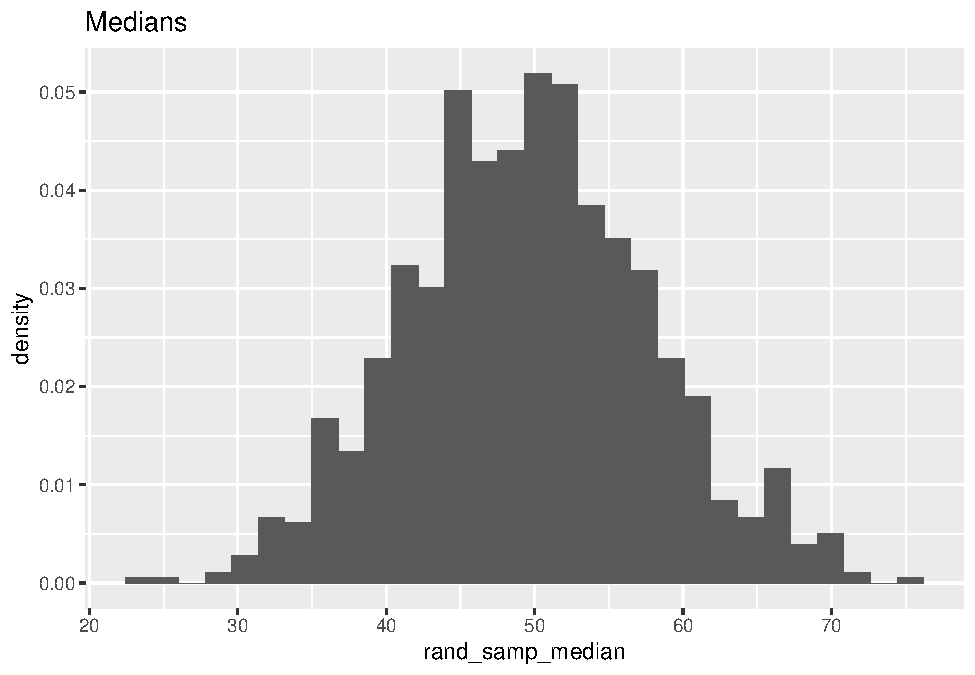
\includegraphics{Class_Exercises_ClassNotes_5_files/figure-latex/unnamed-chunk-5-1.pdf}
\newpage

\begin{Shaded}
\begin{Highlighting}[]
\FunctionTok{ggplot}\NormalTok{(}\AttributeTok{data =} \FunctionTok{data.frame}\NormalTok{(rand\_samp\_sd)) }\SpecialCharTok{+}
  \FunctionTok{geom\_histogram}\NormalTok{(}\AttributeTok{mapping =} \FunctionTok{aes}\NormalTok{(}\AttributeTok{x =}\NormalTok{ rand\_samp\_sd, }\AttributeTok{y =} \FunctionTok{stat}\NormalTok{(density))) }\SpecialCharTok{+}
  \FunctionTok{labs}\NormalTok{(}\AttributeTok{title =} \StringTok{"Standard Deviations"}\NormalTok{)}
\end{Highlighting}
\end{Shaded}

\begin{verbatim}
## `stat_bin()` using `bins = 30`. Pick better value with `binwidth`.
\end{verbatim}

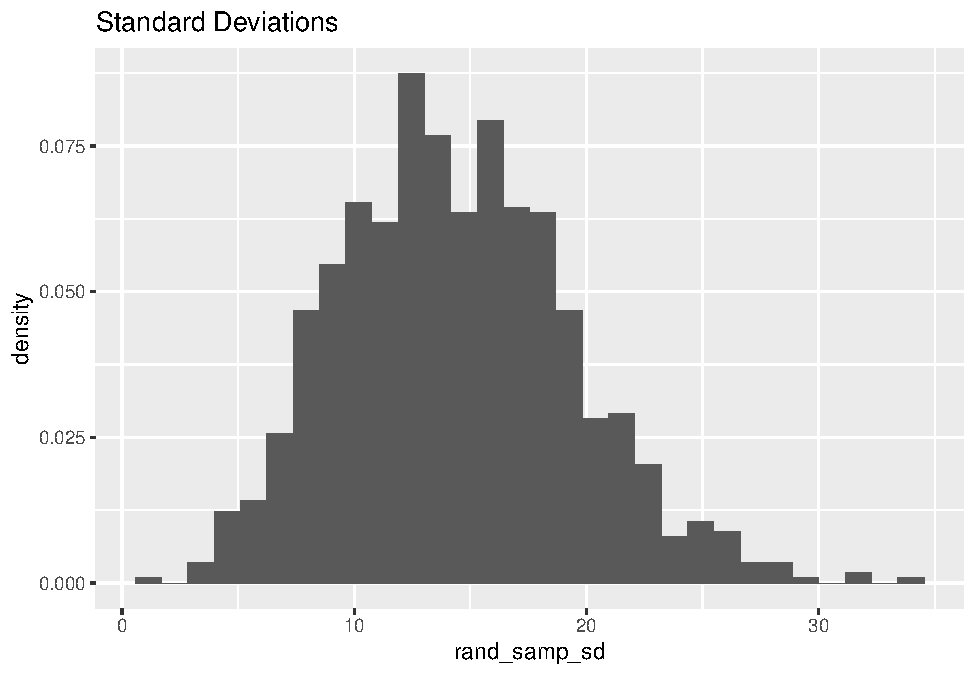
\includegraphics{Class_Exercises_ClassNotes_5_files/figure-latex/unnamed-chunk-6-1.pdf}
\newpage

\begin{Shaded}
\begin{Highlighting}[]
\FunctionTok{ggplot}\NormalTok{(}\AttributeTok{data =} \FunctionTok{data.frame}\NormalTok{(rand\_samp\_min)) }\SpecialCharTok{+}
  \FunctionTok{geom\_histogram}\NormalTok{(}\AttributeTok{mapping =} \FunctionTok{aes}\NormalTok{(}\AttributeTok{x =}\NormalTok{ rand\_samp\_min, }\AttributeTok{y =} \FunctionTok{stat}\NormalTok{(density))) }\SpecialCharTok{+}
  \FunctionTok{labs}\NormalTok{(}\AttributeTok{title =} \StringTok{"Minimums"}\NormalTok{)}
\end{Highlighting}
\end{Shaded}

\begin{verbatim}
## `stat_bin()` using `bins = 30`. Pick better value with `binwidth`.
\end{verbatim}

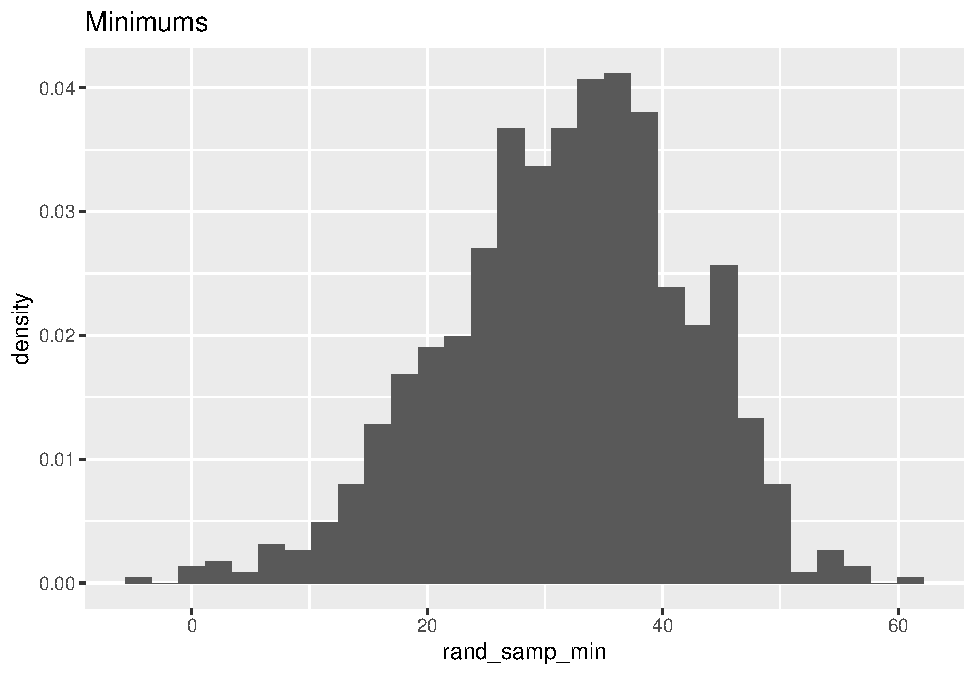
\includegraphics{Class_Exercises_ClassNotes_5_files/figure-latex/unnamed-chunk-7-1.pdf}
\newpage

\begin{Shaded}
\begin{Highlighting}[]
\FunctionTok{ggplot}\NormalTok{(}\AttributeTok{data =} \FunctionTok{data.frame}\NormalTok{(rand\_samp\_max)) }\SpecialCharTok{+}
  \FunctionTok{geom\_histogram}\NormalTok{(}\AttributeTok{mapping =} \FunctionTok{aes}\NormalTok{(}\AttributeTok{x =}\NormalTok{ rand\_samp\_max, }\AttributeTok{y =} \FunctionTok{stat}\NormalTok{(density))) }\SpecialCharTok{+}
  \FunctionTok{labs}\NormalTok{(}\AttributeTok{title =} \StringTok{"Maximums"}\NormalTok{)}
\end{Highlighting}
\end{Shaded}

\begin{verbatim}
## `stat_bin()` using `bins = 30`. Pick better value with `binwidth`.
\end{verbatim}

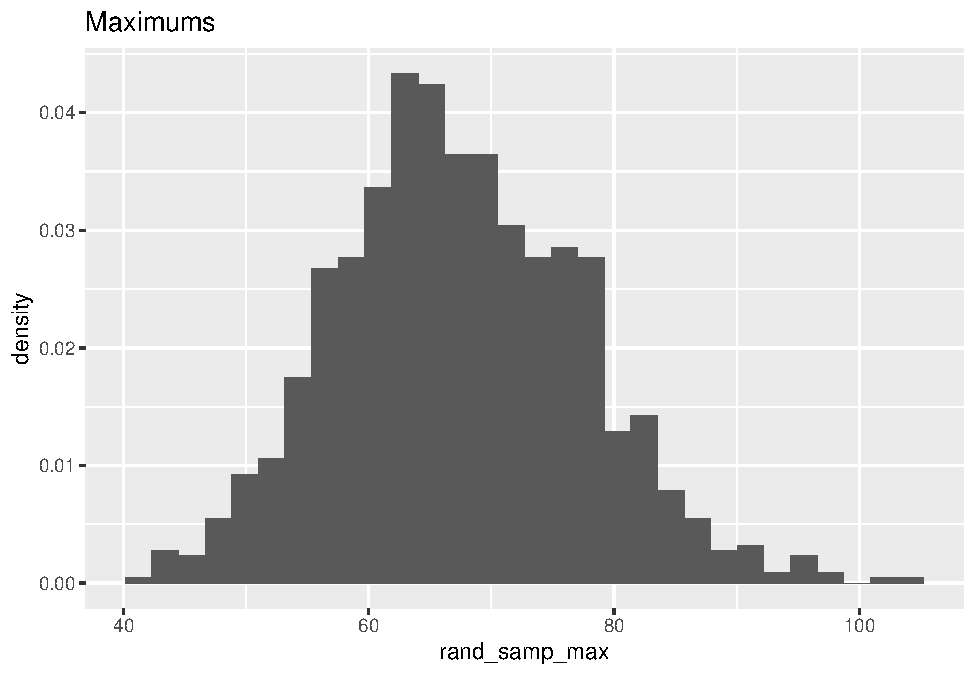
\includegraphics{Class_Exercises_ClassNotes_5_files/figure-latex/unnamed-chunk-8-1.pdf}

\begin{Shaded}
\begin{Highlighting}[]
\NormalTok{mean.of\_median}
\end{Highlighting}
\end{Shaded}

\begin{verbatim}
## [1] 49.57514
\end{verbatim}

\begin{Shaded}
\begin{Highlighting}[]
\NormalTok{mean.of\_sd}
\end{Highlighting}
\end{Shaded}

\begin{verbatim}
## [1] 14.37469
\end{verbatim}

\begin{Shaded}
\begin{Highlighting}[]
\NormalTok{mean.of\_min}
\end{Highlighting}
\end{Shaded}

\begin{verbatim}
## [1] 31.76712
\end{verbatim}

\begin{Shaded}
\begin{Highlighting}[]
\NormalTok{mean.of\_max}
\end{Highlighting}
\end{Shaded}

\begin{verbatim}
## [1] 67.32334
\end{verbatim}

\begin{Shaded}
\begin{Highlighting}[]
\NormalTok{sd.of\_median}
\end{Highlighting}
\end{Shaded}

\begin{verbatim}
## [1] 8.204169
\end{verbatim}

\begin{Shaded}
\begin{Highlighting}[]
\NormalTok{sd.of\_sd}
\end{Highlighting}
\end{Shaded}

\begin{verbatim}
## [1] 4.999422
\end{verbatim}

\begin{Shaded}
\begin{Highlighting}[]
\NormalTok{sd.of\_min}
\end{Highlighting}
\end{Shaded}

\begin{verbatim}
## [1] 10.08694
\end{verbatim}

\begin{Shaded}
\begin{Highlighting}[]
\NormalTok{sd.of\_max}
\end{Highlighting}
\end{Shaded}

\begin{verbatim}
## [1] 9.944542
\end{verbatim}

\hypertarget{section-9.4-exercises}{%
\subsection{Section 9.4 Exercises}\label{section-9.4-exercises}}

\hypertarget{exercise-3-use-the-bootstrap-method-to-simulate-b-1000-resamples-each-of-size-n-150-from-the-original-iris-data-set-and-using-the-petal.width-variable-compute-the-four-statistics-below-for-each-bootstrap-resample.}{%
\subsubsection{Exercise 3: Use the bootstrap method to simulate B =
1,000 resamples each of size n = 150 from the original iris data set,
and using the Petal.Width variable, compute the four statistics below
for each bootstrap
resample.}\label{exercise-3-use-the-bootstrap-method-to-simulate-b-1000-resamples-each-of-size-n-150-from-the-original-iris-data-set-and-using-the-petal.width-variable-compute-the-four-statistics-below-for-each-bootstrap-resample.}}

Code:

\begin{Shaded}
\begin{Highlighting}[]
\FunctionTok{library}\NormalTok{(dplyr)}
\end{Highlighting}
\end{Shaded}

\begin{verbatim}
## 
## Attaching package: 'dplyr'
\end{verbatim}

\begin{verbatim}
## The following objects are masked from 'package:stats':
## 
##     filter, lag
\end{verbatim}

\begin{verbatim}
## The following objects are masked from 'package:base':
## 
##     intersect, setdiff, setequal, union
\end{verbatim}

\begin{Shaded}
\begin{Highlighting}[]
\NormalTok{n.rows }\OtherTok{\textless{}{-}} \FunctionTok{nrow}\NormalTok{(iris)}
\NormalTok{B }\OtherTok{\textless{}{-}} \DecValTok{1000}
\NormalTok{boot.samp\_medians }\OtherTok{\textless{}{-}} \FunctionTok{rep}\NormalTok{(}\ConstantTok{NA}\NormalTok{, B)}
\NormalTok{boot.samp\_sds }\OtherTok{\textless{}{-}} \FunctionTok{rep}\NormalTok{(}\ConstantTok{NA}\NormalTok{, B)}
\NormalTok{boot.samp\_mins }\OtherTok{\textless{}{-}} \FunctionTok{rep}\NormalTok{(}\ConstantTok{NA}\NormalTok{, B)}
\NormalTok{boot.samp\_maxs }\OtherTok{\textless{}{-}} \FunctionTok{rep}\NormalTok{(}\ConstantTok{NA}\NormalTok{, B)}

\FunctionTok{set.seed}\NormalTok{(}\DecValTok{21}\NormalTok{)}
\end{Highlighting}
\end{Shaded}

\begin{Shaded}
\begin{Highlighting}[]
\ControlFlowTok{for}\NormalTok{ (i }\ControlFlowTok{in} \DecValTok{1}\SpecialCharTok{:}\NormalTok{B) \{}
\NormalTok{  resamp }\OtherTok{\textless{}{-}} \FunctionTok{slice\_sample}\NormalTok{(}\AttributeTok{.data =}\NormalTok{ iris,}
                         \AttributeTok{n =}\NormalTok{ n.rows,}
                         \AttributeTok{replace =} \ConstantTok{TRUE}\NormalTok{)}
\NormalTok{  boot.samp\_medians[i] }\OtherTok{\textless{}{-}} \FunctionTok{median}\NormalTok{(resamp}\SpecialCharTok{$}\NormalTok{Petal.Width)}
\NormalTok{  boot.samp\_sds[i] }\OtherTok{\textless{}{-}} \FunctionTok{sd}\NormalTok{(resamp}\SpecialCharTok{$}\NormalTok{Petal.Width)}
\NormalTok{  boot.samp\_mins[i] }\OtherTok{\textless{}{-}} \FunctionTok{min}\NormalTok{(resamp}\SpecialCharTok{$}\NormalTok{Petal.Width)}
\NormalTok{  boot.samp\_maxs[i] }\OtherTok{\textless{}{-}} \FunctionTok{max}\NormalTok{(resamp}\SpecialCharTok{$}\NormalTok{Petal.Width)}
\NormalTok{\}}

\FunctionTok{ggplot}\NormalTok{(}\AttributeTok{data =} \FunctionTok{data.frame}\NormalTok{(boot.samp\_medians)) }\SpecialCharTok{+}
  \FunctionTok{geom\_histogram}\NormalTok{(}\AttributeTok{mapping =} \FunctionTok{aes}\NormalTok{(}\AttributeTok{x =}\NormalTok{ boot.samp\_medians)) }\SpecialCharTok{+}
  \FunctionTok{labs}\NormalTok{(}\AttributeTok{title =} \StringTok{"Medians"}\NormalTok{)}
\end{Highlighting}
\end{Shaded}

\begin{verbatim}
## `stat_bin()` using `bins = 30`. Pick better value with `binwidth`.
\end{verbatim}

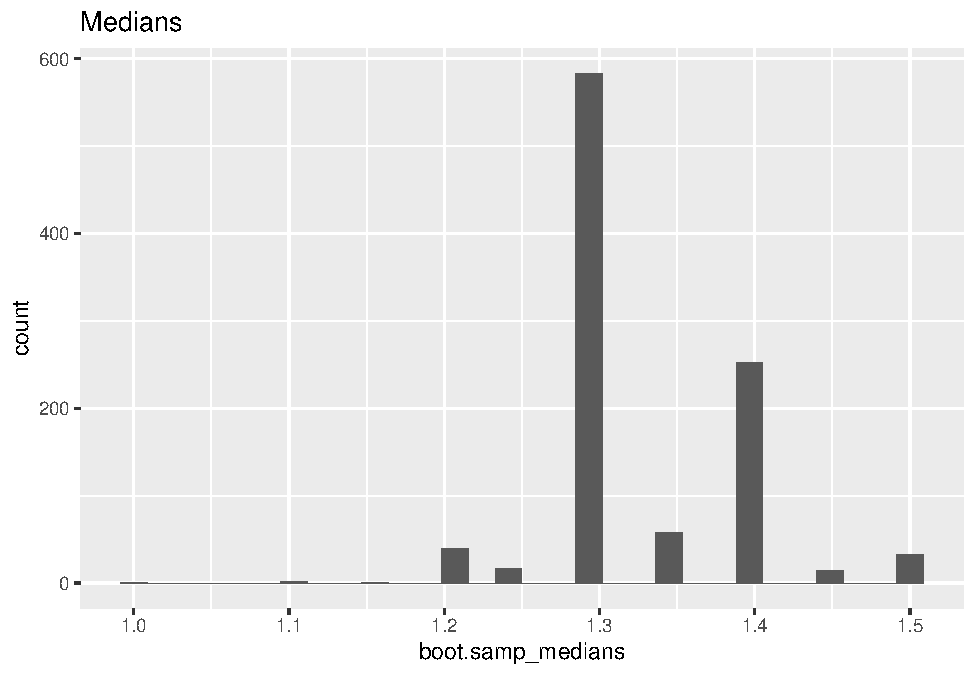
\includegraphics{Class_Exercises_ClassNotes_5_files/figure-latex/unnamed-chunk-10-1.pdf}
\newpage

\begin{Shaded}
\begin{Highlighting}[]
\FunctionTok{ggplot}\NormalTok{(}\AttributeTok{data =} \FunctionTok{data.frame}\NormalTok{(boot.samp\_sds)) }\SpecialCharTok{+}
  \FunctionTok{geom\_histogram}\NormalTok{(}\AttributeTok{mapping =} \FunctionTok{aes}\NormalTok{(}\AttributeTok{x =}\NormalTok{ boot.samp\_sds)) }\SpecialCharTok{+}
  \FunctionTok{labs}\NormalTok{(}\AttributeTok{title =} \StringTok{"Standard Deviations"}\NormalTok{)}
\end{Highlighting}
\end{Shaded}

\begin{verbatim}
## `stat_bin()` using `bins = 30`. Pick better value with `binwidth`.
\end{verbatim}

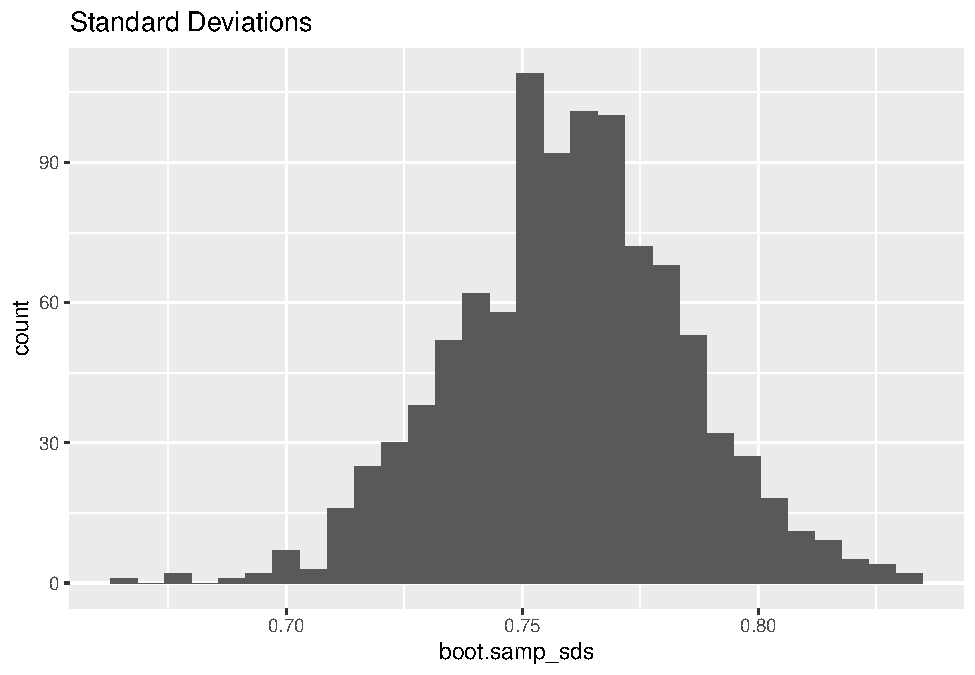
\includegraphics{Class_Exercises_ClassNotes_5_files/figure-latex/unnamed-chunk-11-1.pdf}
\newpage

\begin{Shaded}
\begin{Highlighting}[]
\FunctionTok{ggplot}\NormalTok{(}\AttributeTok{data =} \FunctionTok{data.frame}\NormalTok{(boot.samp\_mins)) }\SpecialCharTok{+}
  \FunctionTok{geom\_histogram}\NormalTok{(}\AttributeTok{mapping =} \FunctionTok{aes}\NormalTok{(}\AttributeTok{x =}\NormalTok{ boot.samp\_mins)) }\SpecialCharTok{+}
  \FunctionTok{labs}\NormalTok{(}\AttributeTok{title =} \StringTok{"Minimums"}\NormalTok{)}
\end{Highlighting}
\end{Shaded}

\begin{verbatim}
## `stat_bin()` using `bins = 30`. Pick better value with `binwidth`.
\end{verbatim}

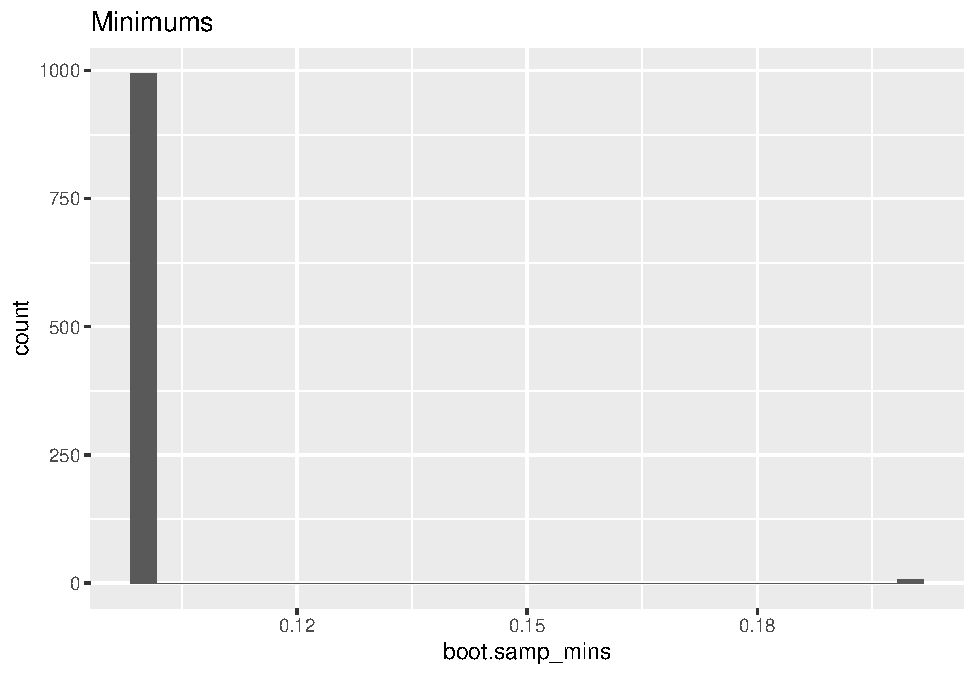
\includegraphics{Class_Exercises_ClassNotes_5_files/figure-latex/unnamed-chunk-12-1.pdf}
\newpage

\begin{Shaded}
\begin{Highlighting}[]
\FunctionTok{ggplot}\NormalTok{(}\AttributeTok{data =} \FunctionTok{data.frame}\NormalTok{(boot.samp\_maxs)) }\SpecialCharTok{+}
  \FunctionTok{geom\_histogram}\NormalTok{(}\AttributeTok{mapping =} \FunctionTok{aes}\NormalTok{(}\AttributeTok{x =}\NormalTok{ boot.samp\_maxs)) }\SpecialCharTok{+}
  \FunctionTok{labs}\NormalTok{(}\AttributeTok{title =} \StringTok{"Maximums"}\NormalTok{)}
\end{Highlighting}
\end{Shaded}

\begin{verbatim}
## `stat_bin()` using `bins = 30`. Pick better value with `binwidth`.
\end{verbatim}

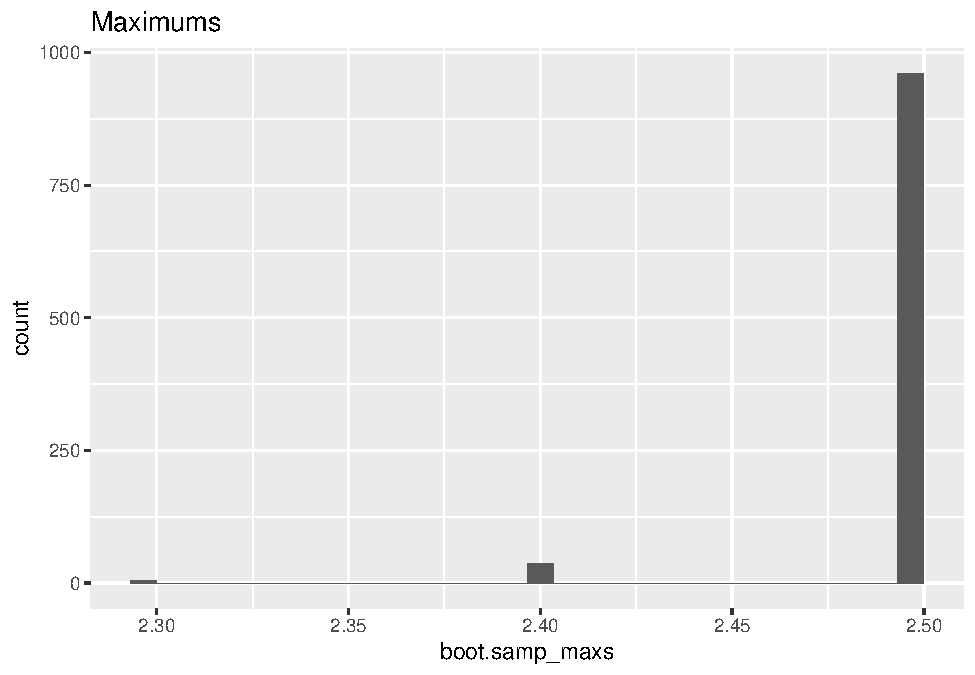
\includegraphics{Class_Exercises_ClassNotes_5_files/figure-latex/unnamed-chunk-13-1.pdf}

\begin{Shaded}
\begin{Highlighting}[]
\NormalTok{median.mean }\OtherTok{\textless{}{-}} \FunctionTok{mean}\NormalTok{(boot.samp\_medians)}
\NormalTok{sd.mean }\OtherTok{\textless{}{-}} \FunctionTok{mean}\NormalTok{(boot.samp\_sds)}
\NormalTok{min.mean }\OtherTok{\textless{}{-}} \FunctionTok{mean}\NormalTok{(boot.samp\_mins)}
\NormalTok{max.mean }\OtherTok{\textless{}{-}} \FunctionTok{mean}\NormalTok{(boot.samp\_maxs)}

\NormalTok{median.sd }\OtherTok{\textless{}{-}} \FunctionTok{sd}\NormalTok{(boot.samp\_medians)}
\NormalTok{sd.sd }\OtherTok{\textless{}{-}} \FunctionTok{sd}\NormalTok{(boot.samp\_sds)}
\NormalTok{min.sd }\OtherTok{\textless{}{-}} \FunctionTok{sd}\NormalTok{(boot.samp\_mins)}
\NormalTok{max.sd }\OtherTok{\textless{}{-}} \FunctionTok{sd}\NormalTok{(boot.samp\_maxs)}

\NormalTok{median.mean}
\end{Highlighting}
\end{Shaded}

\begin{verbatim}
## [1] 1.3312
\end{verbatim}

\begin{Shaded}
\begin{Highlighting}[]
\NormalTok{sd.mean}
\end{Highlighting}
\end{Shaded}

\begin{verbatim}
## [1] 0.7598777
\end{verbatim}

\begin{Shaded}
\begin{Highlighting}[]
\NormalTok{min.mean}
\end{Highlighting}
\end{Shaded}

\begin{verbatim}
## [1] 0.1006
\end{verbatim}

\begin{Shaded}
\begin{Highlighting}[]
\NormalTok{max.mean}
\end{Highlighting}
\end{Shaded}

\begin{verbatim}
## [1] 2.4956
\end{verbatim}

\begin{Shaded}
\begin{Highlighting}[]
\NormalTok{median.sd}
\end{Highlighting}
\end{Shaded}

\begin{verbatim}
## [1] 0.06289289
\end{verbatim}

\begin{Shaded}
\begin{Highlighting}[]
\NormalTok{sd.sd}
\end{Highlighting}
\end{Shaded}

\begin{verbatim}
## [1] 0.02445273
\end{verbatim}

\begin{Shaded}
\begin{Highlighting}[]
\NormalTok{min.sd}
\end{Highlighting}
\end{Shaded}

\begin{verbatim}
## [1] 0.007726558
\end{verbatim}

\begin{Shaded}
\begin{Highlighting}[]
\NormalTok{max.sd}
\end{Highlighting}
\end{Shaded}

\begin{verbatim}
## [1] 0.02238618
\end{verbatim}

\hypertarget{section-9.5-exercises}{%
\subsection{Section 9.5 Exercises}\label{section-9.5-exercises}}

\hypertarget{exercise-4-do-the-following.}{%
\subsubsection{Exercise 4: Do the
following.}\label{exercise-4-do-the-following.}}

Dataframe:

\begin{Shaded}
\begin{Highlighting}[]
\NormalTok{SnakeID }\OtherTok{\textless{}{-}} \DecValTok{1}\SpecialCharTok{:}\DecValTok{10}
\NormalTok{Ln }\OtherTok{\textless{}{-}} \FunctionTok{c}\NormalTok{(}\FloatTok{85.7}\NormalTok{, }\FloatTok{64.5}\NormalTok{, }\FloatTok{84.1}\NormalTok{, }\FloatTok{82.5}\NormalTok{, }\FloatTok{78.0}\NormalTok{, }\FloatTok{65.9}\NormalTok{, }\FloatTok{81.3}\NormalTok{, }\FloatTok{71.0}\NormalTok{, }\FloatTok{86.7}\NormalTok{, }\FloatTok{78.7}\NormalTok{)}
\NormalTok{Wt }\OtherTok{\textless{}{-}}
  \FunctionTok{c}\NormalTok{(}\FloatTok{331.9}\NormalTok{,}
    \FloatTok{121.5}\NormalTok{,}
    \FloatTok{382.2}\NormalTok{,}
    \FloatTok{287.3}\NormalTok{,}
    \FloatTok{224.3}\NormalTok{,}
    \FloatTok{380.4}\NormalTok{,}
    \FloatTok{245.2}\NormalTok{,}
    \FloatTok{208.2}\NormalTok{,}
    \FloatTok{393.4}\NormalTok{,}
    \FloatTok{228.3}\NormalTok{)}
\NormalTok{Snakes }\OtherTok{\textless{}{-}} \FunctionTok{data.frame}\NormalTok{(SnakeID, Ln, Wt)}
\end{Highlighting}
\end{Shaded}

\newpage

\hypertarget{a-can-you-identify-the-outlier-in-either-of-these-univariate-graphs-histograms}{%
\paragraph{a) Can you identify the outlier in either of these univariate
graphs
(histograms)?}\label{a-can-you-identify-the-outlier-in-either-of-these-univariate-graphs-histograms}}

Code:

\begin{Shaded}
\begin{Highlighting}[]
\FunctionTok{ggplot}\NormalTok{(}\AttributeTok{data =}\NormalTok{ Snakes) }\SpecialCharTok{+}
  \FunctionTok{geom\_histogram}\NormalTok{(}
    \AttributeTok{mapping =} \FunctionTok{aes}\NormalTok{(}\AttributeTok{x =}\NormalTok{ Ln),}
    \AttributeTok{fill =} \StringTok{"blue"}\NormalTok{,}
    \AttributeTok{color =} \StringTok{"white"}\NormalTok{,}
    \AttributeTok{bins =} \DecValTok{5}
\NormalTok{  ) }\SpecialCharTok{+}
  \FunctionTok{ggtitle}\NormalTok{(}\StringTok{"Histogram of Snakes Lengths"}\NormalTok{)}
\end{Highlighting}
\end{Shaded}

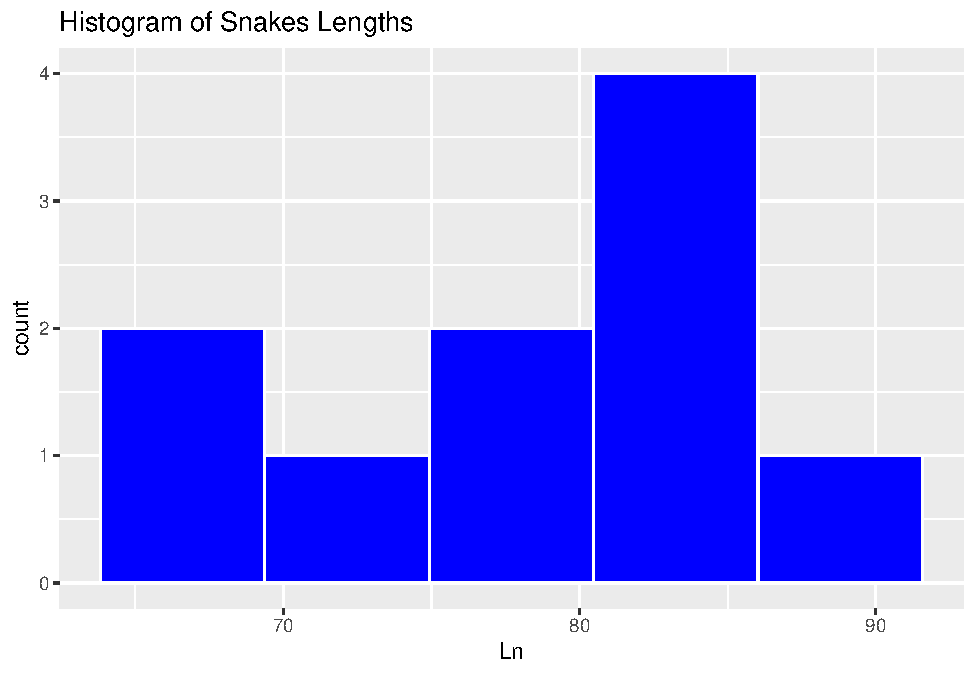
\includegraphics{Class_Exercises_ClassNotes_5_files/figure-latex/unnamed-chunk-15-1.pdf}
\newpage

\begin{Shaded}
\begin{Highlighting}[]
\FunctionTok{ggplot}\NormalTok{(}\AttributeTok{data =}\NormalTok{ Snakes) }\SpecialCharTok{+}
  \FunctionTok{geom\_histogram}\NormalTok{(}
    \AttributeTok{mapping =} \FunctionTok{aes}\NormalTok{(}\AttributeTok{x =}\NormalTok{ Wt),}
    \AttributeTok{fill =} \StringTok{"blue"}\NormalTok{,}
    \AttributeTok{color =} \StringTok{"white"}\NormalTok{,}
    \AttributeTok{bins =} \DecValTok{5}
\NormalTok{  ) }\SpecialCharTok{+}
  \FunctionTok{ggtitle}\NormalTok{(}\StringTok{"Histogram of Snakes Weights"}\NormalTok{)}
\end{Highlighting}
\end{Shaded}

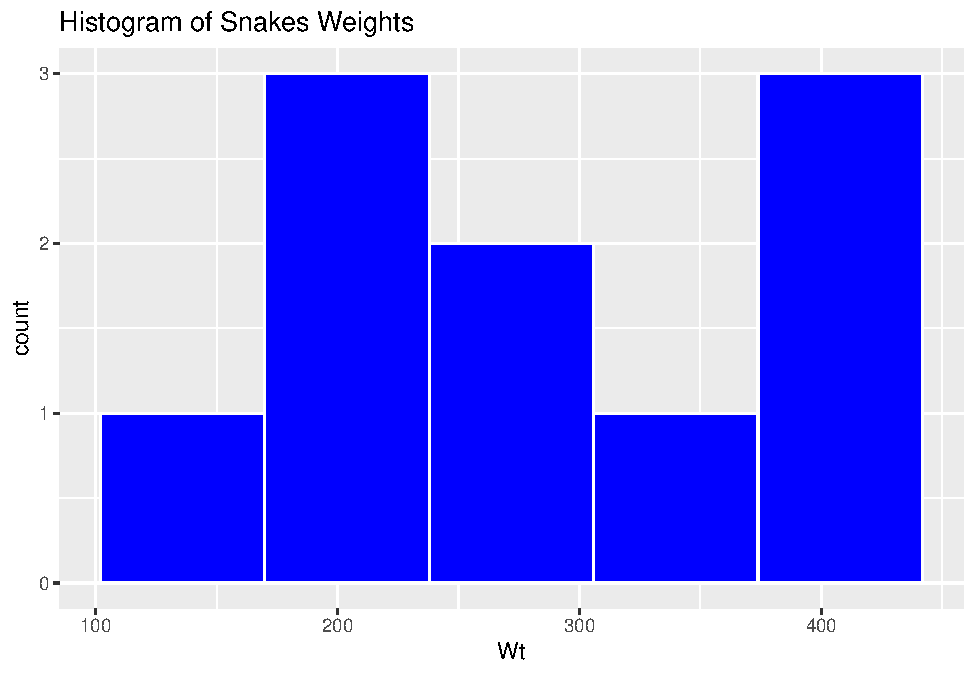
\includegraphics{Class_Exercises_ClassNotes_5_files/figure-latex/unnamed-chunk-16-1.pdf}
The only outlier in the two graphs is the weight of the snakes. The
outlier value is 121.5. \newpage

\hypertarget{b-can-you-identify-the-outlier-in-this-bivariate-graph-scatterplot-if-so-which-snake-snakeid-is-the-outlier}{%
\paragraph{b) Can you identify the outlier in this bivariate graph
(scatterplot)? If so, which snake (SnakeID) is the
outlier?}\label{b-can-you-identify-the-outlier-in-this-bivariate-graph-scatterplot-if-so-which-snake-snakeid-is-the-outlier}}

Code:

\begin{Shaded}
\begin{Highlighting}[]
\FunctionTok{ggplot}\NormalTok{(}\AttributeTok{data =}\NormalTok{ Snakes) }\SpecialCharTok{+}
  \FunctionTok{geom\_point}\NormalTok{(}\AttributeTok{mapping =} \FunctionTok{aes}\NormalTok{(}\AttributeTok{x =}\NormalTok{ Ln, }\AttributeTok{y =}\NormalTok{ Wt)) }\SpecialCharTok{+}
  \FunctionTok{ggtitle}\NormalTok{(}\StringTok{"Scatterplot of Weights vs Lengths"}\NormalTok{)}
\end{Highlighting}
\end{Shaded}

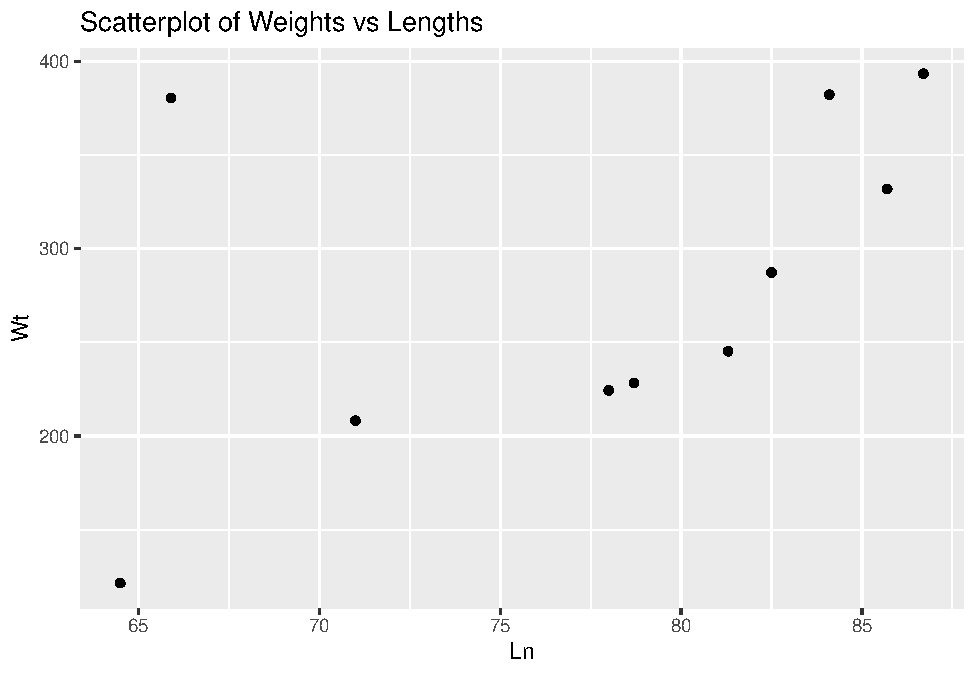
\includegraphics{Class_Exercises_ClassNotes_5_files/figure-latex/unnamed-chunk-17-1.pdf}
The major outlier is the snake whose length is 65.9 with a weight of
380.4 and the second most significant outlier is the snake with a 64.5
length and a 121.5 weight. \newpage

\hypertarget{section-9.6-exercises}{%
\subsection{Section 9.6 Exercises}\label{section-9.6-exercises}}

\hypertarget{exercise-5-do-the-following.}{%
\subsubsection{Exercise 5: Do the
following.}\label{exercise-5-do-the-following.}}

Data frame:

\begin{Shaded}
\begin{Highlighting}[]
\NormalTok{SnakeID }\OtherTok{\textless{}{-}} \DecValTok{1}\SpecialCharTok{:}\DecValTok{9}
\NormalTok{Ln }\OtherTok{\textless{}{-}} \FunctionTok{c}\NormalTok{(}\FloatTok{85.7}\NormalTok{, }\FloatTok{64.5}\NormalTok{, }\FloatTok{84.1}\NormalTok{, }\FloatTok{82.5}\NormalTok{, }\FloatTok{78.0}\NormalTok{, }\FloatTok{81.3}\NormalTok{, }\FloatTok{71.0}\NormalTok{, }\FloatTok{86.7}\NormalTok{, }\FloatTok{78.7}\NormalTok{)}
\NormalTok{Wt }\OtherTok{\textless{}{-}}
  \FunctionTok{c}\NormalTok{(}\FloatTok{331.9}\NormalTok{, }\FloatTok{121.5}\NormalTok{, }\FloatTok{382.2}\NormalTok{, }\FloatTok{287.3}\NormalTok{, }\FloatTok{224.3}\NormalTok{, }\FloatTok{245.2}\NormalTok{, }\FloatTok{208.2}\NormalTok{, }\FloatTok{393.4}\NormalTok{, }\FloatTok{228.3}\NormalTok{)}
\NormalTok{Snakes }\OtherTok{\textless{}{-}} \FunctionTok{data.frame}\NormalTok{(SnakeID, Ln, Wt)}

\FunctionTok{ggplot}\NormalTok{(}\AttributeTok{data =}\NormalTok{ Snakes, }\AttributeTok{mapping =} \FunctionTok{aes}\NormalTok{(}\AttributeTok{x =}\NormalTok{ Ln, }\AttributeTok{y =}\NormalTok{ Wt)) }\SpecialCharTok{+}
  \FunctionTok{geom\_point}\NormalTok{() }\SpecialCharTok{+}
  \FunctionTok{geom\_smooth}\NormalTok{(}\AttributeTok{method =} \StringTok{"lm"}\NormalTok{, }\AttributeTok{se =} \ConstantTok{FALSE}\NormalTok{) }\SpecialCharTok{+}
  \FunctionTok{ggtitle}\NormalTok{(}\StringTok{"Scatterplot of Weights vs Lengths"}\NormalTok{)}
\end{Highlighting}
\end{Shaded}

\begin{verbatim}
## `geom_smooth()` using formula 'y ~ x'
\end{verbatim}

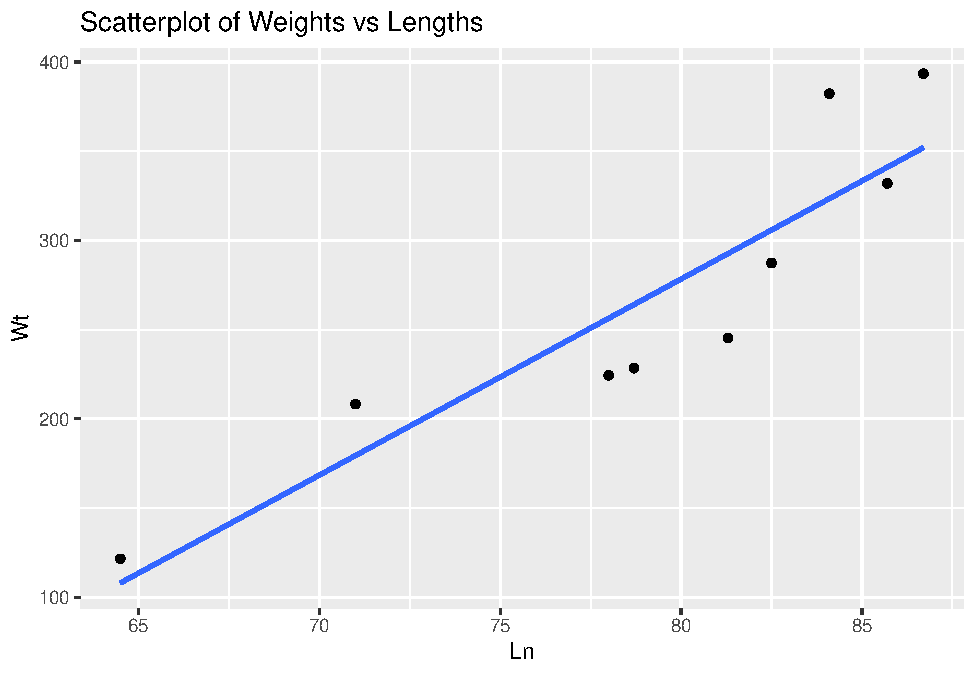
\includegraphics{Class_Exercises_ClassNotes_5_files/figure-latex/unnamed-chunk-18-1.pdf}
\newpage

\begin{Shaded}
\begin{Highlighting}[]
\NormalTok{my.reg }\OtherTok{\textless{}{-}} \FunctionTok{lm}\NormalTok{(Wt }\SpecialCharTok{\textasciitilde{}}\NormalTok{ Ln, }\AttributeTok{data =}\NormalTok{ Snakes)}
\FunctionTok{summary}\NormalTok{(my.reg)}
\end{Highlighting}
\end{Shaded}

\begin{verbatim}
## 
## Call:
## lm(formula = Wt ~ Ln, data = Snakes)
## 
## Residuals:
##     Min      1Q  Median      3Q     Max 
## -47.395 -32.020  -9.061  28.826  58.827 
## 
## Coefficients:
##             Estimate Std. Error t value Pr(>|t|)    
## (Intercept) -601.083    154.333  -3.895 0.005939 ** 
## Ln            10.992      1.942   5.660 0.000767 ***
## ---
## Signif. codes:  0 '***' 0.001 '**' 0.01 '*' 0.05 '.' 0.1 ' ' 1
## 
## Residual standard error: 39.94 on 7 degrees of freedom
## Multiple R-squared:  0.8207, Adjusted R-squared:  0.795 
## F-statistic: 32.03 on 1 and 7 DF,  p-value: 0.0007667
\end{verbatim}

\hypertarget{a-obtain-the-predicted-weight-for-a-snake-whose-length-is-80-cm-in-two-ways}{%
\paragraph{a) Obtain the predicted weight for a snake whose length is 80
cm in two
ways:}\label{a-obtain-the-predicted-weight-for-a-snake-whose-length-is-80-cm-in-two-ways}}

\begin{enumerate}
\def\labelenumi{\arabic{enumi}.}
\tightlist
\item
  By plugging 80 into the equation for X.
\item
  By using predict(). Report both sets of your R commands for obtaining
  the predicted weight.\\
  Code:
\end{enumerate}

\begin{Shaded}
\begin{Highlighting}[]
\NormalTok{pred\_val }\OtherTok{\textless{}{-}} \SpecialCharTok{{-}}\FloatTok{601.08} \SpecialCharTok{+} \FloatTok{10.99} \SpecialCharTok{*} \DecValTok{80}
\NormalTok{pred\_val}
\end{Highlighting}
\end{Shaded}

\begin{verbatim}
## [1] 278.12
\end{verbatim}

\begin{Shaded}
\begin{Highlighting}[]
\NormalTok{newLen }\OtherTok{\textless{}{-}} \FunctionTok{data.frame}\NormalTok{(}\AttributeTok{Ln =} \DecValTok{80}\NormalTok{)}
\FunctionTok{predict}\NormalTok{(my.reg, }\AttributeTok{newdata =}\NormalTok{ newLen)}
\end{Highlighting}
\end{Shaded}

\begin{verbatim}
##        1 
## 278.3047
\end{verbatim}

\hypertarget{b-whats-a-typical-change-in-weight-for-each-1-cm-elongation-what-about-for-a-5-cm-elongation}{%
\paragraph{b) What's a typical change in weight for each 1 cm
elongation? What about for a 5 cm
elongation?}\label{b-whats-a-typical-change-in-weight-for-each-1-cm-elongation-what-about-for-a-5-cm-elongation}}

\hfill\break
Code:

\begin{Shaded}
\begin{Highlighting}[]
\NormalTok{newLen }\OtherTok{\textless{}{-}} \FunctionTok{data.frame}\NormalTok{(}\AttributeTok{Ln =} \FunctionTok{c}\NormalTok{(}\DecValTok{80}\NormalTok{, }\DecValTok{81}\NormalTok{))}
\FunctionTok{predict}\NormalTok{(my.reg, }\AttributeTok{newdata =}\NormalTok{ newLen)}
\end{Highlighting}
\end{Shaded}

\begin{verbatim}
##        1        2 
## 278.3047 289.2971
\end{verbatim}

For every centimeter change in length, the weight should increase by
approximately 11 and for five cm it should be approximately 55.

\hypertarget{exercise-6-do-the-following.}{%
\subsubsection{Exercise 6: Do the
following.}\label{exercise-6-do-the-following.}}

\hfill\break
Data frame:

\begin{Shaded}
\begin{Highlighting}[]
\FunctionTok{library}\NormalTok{(nycflights13)}
\NormalTok{SF }\OtherTok{\textless{}{-}} \FunctionTok{filter}\NormalTok{(}\AttributeTok{.data =}\NormalTok{ flights, dest }\SpecialCharTok{==} \StringTok{"SFO"}\NormalTok{, }\SpecialCharTok{!}\FunctionTok{is.na}\NormalTok{(arr\_delay))}

\FunctionTok{ggplot}\NormalTok{(}\AttributeTok{data =}\NormalTok{ SF, }\AttributeTok{mapping =} \FunctionTok{aes}\NormalTok{(}\AttributeTok{x =}\NormalTok{ hour, }\AttributeTok{y =}\NormalTok{ dep\_delay)) }\SpecialCharTok{+}
  \FunctionTok{geom\_point}\NormalTok{() }\SpecialCharTok{+}
  \FunctionTok{geom\_smooth}\NormalTok{(}\AttributeTok{method =} \StringTok{"lm"}\NormalTok{) }\SpecialCharTok{+}
  \FunctionTok{xlab}\NormalTok{(}\StringTok{"Scheduled Hour of Departure"}\NormalTok{) }\SpecialCharTok{+}     \FunctionTok{ylab}\NormalTok{(}\StringTok{"Departure Delay (Minutes)"}\NormalTok{) }\SpecialCharTok{+}
  \FunctionTok{coord\_cartesian}\NormalTok{(}\AttributeTok{ylim =} \FunctionTok{c}\NormalTok{(}\SpecialCharTok{{-}}\DecValTok{30}\NormalTok{, }\DecValTok{200}\NormalTok{))}
\end{Highlighting}
\end{Shaded}

\begin{verbatim}
## `geom_smooth()` using formula 'y ~ x'
\end{verbatim}

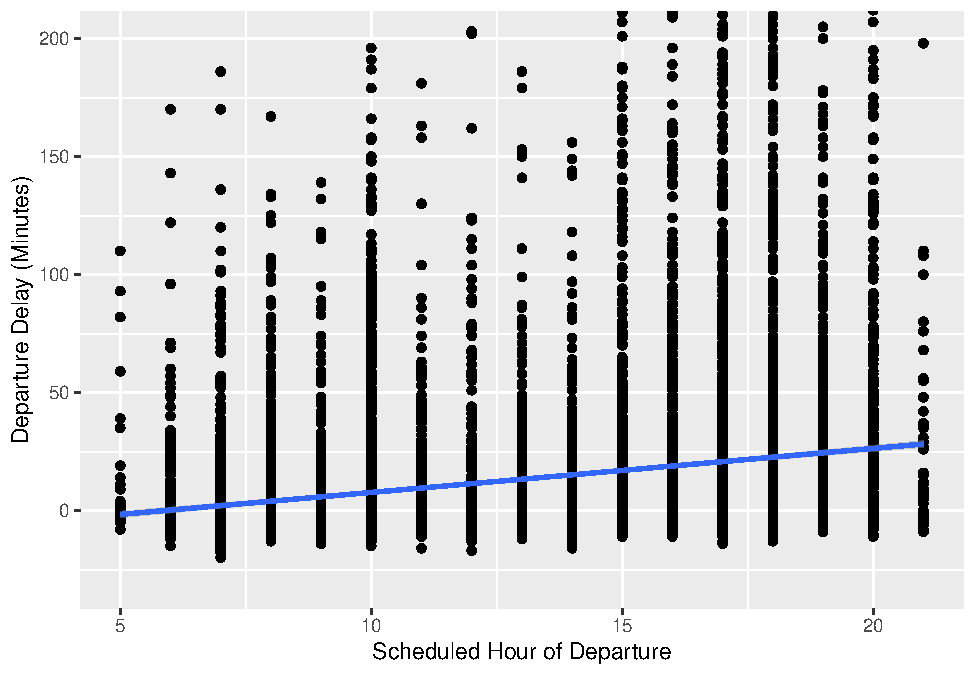
\includegraphics{Class_Exercises_ClassNotes_5_files/figure-latex/unnamed-chunk-22-1.pdf}
\newpage

\hypertarget{a-use-lm-and-summary-to-obtain-the-equation-of-the-fitted-regression-line-with-with-dep_delay-as-the-response-y-and-hour-as-the-explanatory-variable-x.-report-the-equation-of-the-fitted-line.}{%
\paragraph{a) Use lm() and summary() to obtain the equation of the
fitted regression line, with with dep\_delay as the response (Y ) and
hour as the explanatory variable (X). Report the equation of the fitted
line.}\label{a-use-lm-and-summary-to-obtain-the-equation-of-the-fitted-regression-line-with-with-dep_delay-as-the-response-y-and-hour-as-the-explanatory-variable-x.-report-the-equation-of-the-fitted-line.}}

\hfill\break
Code:

\begin{Shaded}
\begin{Highlighting}[]
\NormalTok{my.reg2 }\OtherTok{\textless{}{-}} \FunctionTok{lm}\NormalTok{(dep\_delay }\SpecialCharTok{\textasciitilde{}}\NormalTok{ hour, }\AttributeTok{data =}\NormalTok{ SF)}
\FunctionTok{summary}\NormalTok{(my.reg2)}
\end{Highlighting}
\end{Shaded}

\begin{verbatim}
## 
## Call:
## lm(formula = dep_delay ~ hour, data = SF)
## 
## Residuals:
##    Min     1Q Median     3Q    Max 
## -37.33 -17.42  -8.74  -1.10 991.39 
## 
## Coefficients:
##              Estimate Std. Error t value Pr(>|t|)    
## (Intercept) -10.95593    1.03591  -10.58   <2e-16 ***
## hour          1.86451    0.07692   24.24   <2e-16 ***
## ---
## Signif. codes:  0 '***' 0.001 '**' 0.01 '*' 0.05 '.' 0.1 ' ' 1
## 
## Residual standard error: 39.34 on 13171 degrees of freedom
## Multiple R-squared:  0.0427, Adjusted R-squared:  0.04263 
## F-statistic: 587.5 on 1 and 13171 DF,  p-value: < 2.2e-16
\end{verbatim}

The equation of the fitted line is Y = -10.95593 + 1.86451X.

\hypertarget{b-obtain-the-predicted-departure-delay-for-a-flight-whose-departure-hour-is-15-in-two-ways}{%
\paragraph{b) Obtain the predicted departure delay for a flight whose
departure hour is 15 in two
ways:}\label{b-obtain-the-predicted-departure-delay-for-a-flight-whose-departure-hour-is-15-in-two-ways}}

\begin{enumerate}
\def\labelenumi{\arabic{enumi}.}
\tightlist
\item
  By plugging 15 into the equation for X.
\item
  By using predict(). Report both sets of your R commands for obtaining
  the predicted departure delay.\\
  Code:
\end{enumerate}

\begin{Shaded}
\begin{Highlighting}[]
\SpecialCharTok{{-}}\FloatTok{10.95593} \SpecialCharTok{+} \FloatTok{1.86451} \SpecialCharTok{*} \DecValTok{15}
\end{Highlighting}
\end{Shaded}

\begin{verbatim}
## [1] 17.01172
\end{verbatim}

\begin{Shaded}
\begin{Highlighting}[]
\NormalTok{newHour }\OtherTok{\textless{}{-}} \FunctionTok{data.frame}\NormalTok{(}\AttributeTok{hour =} \DecValTok{15}\NormalTok{)}
\FunctionTok{predict}\NormalTok{(my.reg2, }\AttributeTok{newdata =}\NormalTok{ newHour)}
\end{Highlighting}
\end{Shaded}

\begin{verbatim}
##        1 
## 17.01166
\end{verbatim}

The departure delay will increase by 1.86451 for each hour that is
additional.

\hypertarget{section-9.6-exercises-1}{%
\subsection{Section 9.6 Exercises}\label{section-9.6-exercises-1}}

\hypertarget{exercise-7-do-the-following.}{%
\subsubsection{Exercise 7: Do the
following.}\label{exercise-7-do-the-following.}}

\hfill\break
Data frame:

\begin{Shaded}
\begin{Highlighting}[]
\NormalTok{SnakeID }\OtherTok{\textless{}{-}} \DecValTok{1}\SpecialCharTok{:}\DecValTok{9}
\NormalTok{Ln }\OtherTok{\textless{}{-}} \FunctionTok{c}\NormalTok{(}\FloatTok{85.7}\NormalTok{, }\FloatTok{64.5}\NormalTok{, }\FloatTok{84.1}\NormalTok{, }\FloatTok{82.5}\NormalTok{, }\FloatTok{78.0}\NormalTok{, }\FloatTok{81.3}\NormalTok{, }\FloatTok{71.0}\NormalTok{, }\FloatTok{86.7}\NormalTok{, }\FloatTok{78.7}\NormalTok{)}
\NormalTok{Wt }\OtherTok{\textless{}{-}}
  \FunctionTok{c}\NormalTok{(}\FloatTok{331.9}\NormalTok{, }\FloatTok{121.5}\NormalTok{, }\FloatTok{382.2}\NormalTok{, }\FloatTok{287.3}\NormalTok{, }\FloatTok{224.3}\NormalTok{, }\FloatTok{245.2}\NormalTok{, }\FloatTok{208.2}\NormalTok{, }\FloatTok{393.4}\NormalTok{, }\FloatTok{228.3}\NormalTok{)}
\NormalTok{Snakes }\OtherTok{\textless{}{-}} \FunctionTok{data.frame}\NormalTok{(SnakeID, Ln, Wt)}
\NormalTok{my.reg }\OtherTok{\textless{}{-}} \FunctionTok{lm}\NormalTok{(Wt }\SpecialCharTok{\textasciitilde{}}\NormalTok{ Ln, }\AttributeTok{data =}\NormalTok{ Snakes)}
\end{Highlighting}
\end{Shaded}

\hypertarget{a-what-class-of-object-is-returned-by-lm-find-out-by-typing}{%
\paragraph{a) What class of object is returned by lm()? Find out by
typing:}\label{a-what-class-of-object-is-returned-by-lm-find-out-by-typing}}

\hfill\break
Code:

\begin{Shaded}
\begin{Highlighting}[]
\FunctionTok{class}\NormalTok{(my.reg)}
\end{Highlighting}
\end{Shaded}

\begin{verbatim}
## [1] "lm"
\end{verbatim}

\hypertarget{b-the-lm-class-of-objects-is-a-special-case-of-the-list-class.-what-does-the-following-return}{%
\paragraph{b) The ``lm'' class of objects is a special case of the
``list'' class. What does the following
return?}\label{b-the-lm-class-of-objects-is-a-special-case-of-the-list-class.-what-does-the-following-return}}

\hfill\break
Code:

\begin{Shaded}
\begin{Highlighting}[]
\FunctionTok{is.list}\NormalTok{(my.reg)}
\end{Highlighting}
\end{Shaded}

\begin{verbatim}
## [1] TRUE
\end{verbatim}

\hypertarget{c-how-many-objects-are-contained-in-the-my.reg-list-find-out-by-looking-at-their-names}{%
\paragraph{c) How many objects are contained in the my.reg list? Find
out by looking at their
names:}\label{c-how-many-objects-are-contained-in-the-my.reg-list-find-out-by-looking-at-their-names}}

\hfill\break
Code:

\begin{Shaded}
\begin{Highlighting}[]
\FunctionTok{names}\NormalTok{(my.reg)}
\end{Highlighting}
\end{Shaded}

\begin{verbatim}
##  [1] "coefficients"  "residuals"     "effects"       "rank"         
##  [5] "fitted.values" "assign"        "qr"            "df.residual"  
##  [9] "xlevels"       "call"          "terms"         "model"
\end{verbatim}

\hypertarget{d-what-would-a-plot-of-the-fitted-values-versus-the-lengths-look-like-try-it-and-describe-the-result}{%
\paragraph{d) What would a plot of the fitted values versus the lengths
look like? Try it, and describe the
result:}\label{d-what-would-a-plot-of-the-fitted-values-versus-the-lengths-look-like-try-it-and-describe-the-result}}

\hfill\break
Code:

\begin{Shaded}
\begin{Highlighting}[]
\FunctionTok{library}\NormalTok{(dplyr) }\CommentTok{\# For mutate()}
\NormalTok{Snakes }\OtherTok{\textless{}{-}} \FunctionTok{mutate}\NormalTok{(Snakes, }\AttributeTok{FittedVals =}\NormalTok{ my.reg}\SpecialCharTok{$}\NormalTok{fitted.values)}
\FunctionTok{ggplot}\NormalTok{(}\AttributeTok{data =}\NormalTok{ Snakes, }\AttributeTok{mapping =} \FunctionTok{aes}\NormalTok{(}\AttributeTok{x =}\NormalTok{ Ln, }\AttributeTok{y =}\NormalTok{ FittedVals)) }\SpecialCharTok{+}
  \FunctionTok{geom\_point}\NormalTok{() }\SpecialCharTok{+}
  \FunctionTok{ggtitle}\NormalTok{(}\StringTok{"Scatterplot of Fitted Values vs Lengths"}\NormalTok{)}
\end{Highlighting}
\end{Shaded}

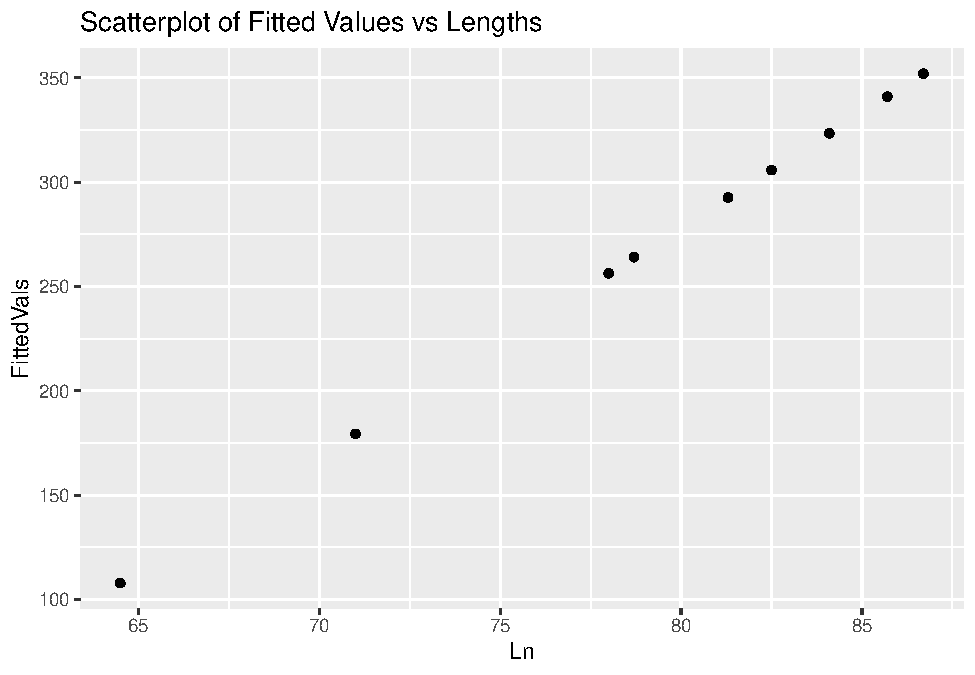
\includegraphics{Class_Exercises_ClassNotes_5_files/figure-latex/unnamed-chunk-29-1.pdf}
The output is almost a perfect linear representation of the snakes data.
\newpage

\hypertarget{e-what-would-a-plot-of-the-residuals-versus-the-lengths-look-like-try-it-with-a-horizontal-line-at-y-0-and-describe-the-result}{%
\paragraph{e) What would a plot of the residuals versus the lengths look
like? Try it (with a horizontal line at y = 0) and describe the
result:}\label{e-what-would-a-plot-of-the-residuals-versus-the-lengths-look-like-try-it-with-a-horizontal-line-at-y-0-and-describe-the-result}}

\hfill\break
Code:

\begin{Shaded}
\begin{Highlighting}[]
\NormalTok{Snakes }\OtherTok{\textless{}{-}} \FunctionTok{mutate}\NormalTok{(Snakes, }\AttributeTok{Residuals =}\NormalTok{ my.reg}\SpecialCharTok{$}\NormalTok{residuals)}
\FunctionTok{ggplot}\NormalTok{(}\AttributeTok{data =}\NormalTok{ Snakes, }\AttributeTok{mapping =} \FunctionTok{aes}\NormalTok{(}\AttributeTok{x =}\NormalTok{ Ln, }\AttributeTok{y =}\NormalTok{ Residuals)) }\SpecialCharTok{+}
  \FunctionTok{geom\_point}\NormalTok{() }\SpecialCharTok{+}
  \FunctionTok{geom\_hline}\NormalTok{(}\AttributeTok{yintercept =} \DecValTok{0}\NormalTok{) }\SpecialCharTok{+}
  \FunctionTok{ggtitle}\NormalTok{(}\StringTok{"Scatterplot of Residuals vs Lengths"}\NormalTok{)}
\end{Highlighting}
\end{Shaded}

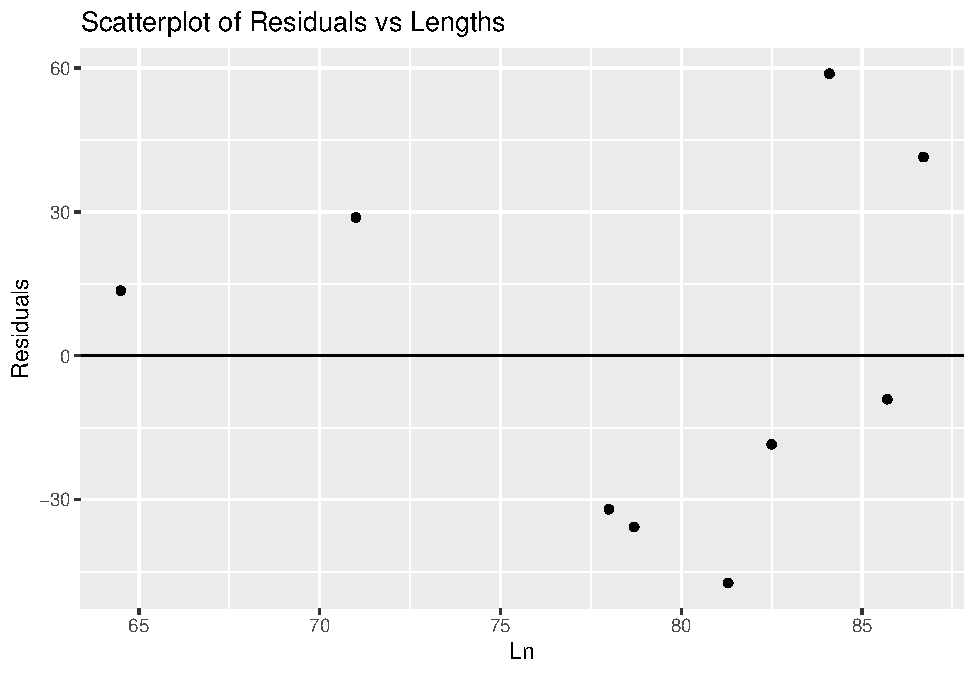
\includegraphics{Class_Exercises_ClassNotes_5_files/figure-latex/unnamed-chunk-30-1.pdf}
The residuals seem pretty far off compared to the horizontal line.

\hypertarget{f-show-that-the-residuals-sum-to-zero}{%
\paragraph{f) Show that the residuals sum to
zero:}\label{f-show-that-the-residuals-sum-to-zero}}

\hfill\break
Code:

\begin{Shaded}
\begin{Highlighting}[]
\FunctionTok{sum}\NormalTok{(Snakes}\SpecialCharTok{$}\NormalTok{Residuals)}
\end{Highlighting}
\end{Shaded}

\begin{verbatim}
## [1] -1.065814e-14
\end{verbatim}

\newpage

\hypertarget{exercise-8-do-the-following.}{%
\subsubsection{Exercise 8: Do the
following.}\label{exercise-8-do-the-following.}}

\hfill\break
Code:

\begin{Shaded}
\begin{Highlighting}[]
\FunctionTok{ggplot}\NormalTok{(}\AttributeTok{data =}\NormalTok{ SF, }\AttributeTok{mapping =} \FunctionTok{aes}\NormalTok{(}\AttributeTok{x =}\NormalTok{ hour, }\AttributeTok{y =}\NormalTok{ dep\_delay)) }\SpecialCharTok{+}
  \FunctionTok{geom\_point}\NormalTok{() }\SpecialCharTok{+}
  \FunctionTok{geom\_smooth}\NormalTok{(}\AttributeTok{method =} \StringTok{"lm"}\NormalTok{) }\SpecialCharTok{+}
  \FunctionTok{xlab}\NormalTok{(}\StringTok{"Scheduled Hour of Departure"}\NormalTok{) }\SpecialCharTok{+} \FunctionTok{ylab}\NormalTok{(}\StringTok{"Departure Delay (Minutes)"}\NormalTok{) }\SpecialCharTok{+}
  \FunctionTok{coord\_cartesian}\NormalTok{(}\AttributeTok{ylim =} \FunctionTok{c}\NormalTok{(}\SpecialCharTok{{-}}\DecValTok{30}\NormalTok{, }\DecValTok{200}\NormalTok{))}
\end{Highlighting}
\end{Shaded}

\begin{verbatim}
## `geom_smooth()` using formula 'y ~ x'
\end{verbatim}

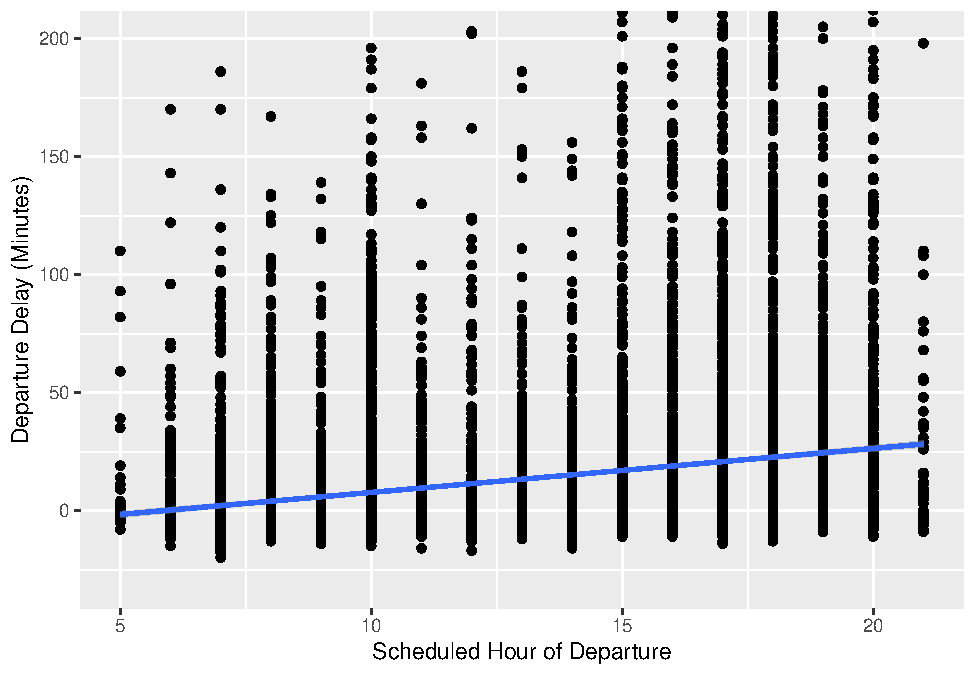
\includegraphics{Class_Exercises_ClassNotes_5_files/figure-latex/unnamed-chunk-32-1.pdf}
\newpage

\begin{Shaded}
\begin{Highlighting}[]
\NormalTok{my.reg }\OtherTok{\textless{}{-}} \FunctionTok{lm}\NormalTok{(dep\_delay }\SpecialCharTok{\textasciitilde{}}\NormalTok{ hour, }\AttributeTok{data =}\NormalTok{ SF)}
\FunctionTok{summary}\NormalTok{(my.reg)}
\end{Highlighting}
\end{Shaded}

\begin{verbatim}
## 
## Call:
## lm(formula = dep_delay ~ hour, data = SF)
## 
## Residuals:
##    Min     1Q Median     3Q    Max 
## -37.33 -17.42  -8.74  -1.10 991.39 
## 
## Coefficients:
##              Estimate Std. Error t value Pr(>|t|)    
## (Intercept) -10.95593    1.03591  -10.58   <2e-16 ***
## hour          1.86451    0.07692   24.24   <2e-16 ***
## ---
## Signif. codes:  0 '***' 0.001 '**' 0.01 '*' 0.05 '.' 0.1 ' ' 1
## 
## Residual standard error: 39.34 on 13171 degrees of freedom
## Multiple R-squared:  0.0427, Adjusted R-squared:  0.04263 
## F-statistic: 587.5 on 1 and 13171 DF,  p-value: < 2.2e-16
\end{verbatim}

\hypertarget{a-from-the-output-of-summary-whats-the-value-of-the-residual-standard-error}{%
\paragraph{a) From the output of summary(), what's the value of the
residual standard
error?}\label{a-from-the-output-of-summary-whats-the-value-of-the-residual-standard-error}}

\hfill\break
The residual standard error is: 39.34.

\hypertarget{b-from-the-output-of-summary-whats-the-value-of-r2-labeled-multiple-r-squared}{%
\paragraph{b) From the output of summary(), what's the value of R2
(labeled Multiple
R-squared)?}\label{b-from-the-output-of-summary-whats-the-value-of-r2-labeled-multiple-r-squared}}

\hfill\break
The value of R2 is 0.0427.

\hypertarget{c-using-the-criteria-below-and-the-r2-from-part-b-how-well-does-the-linear-model-fit-the-data-poor-medium-or-good}{%
\paragraph{c) Using the criteria below (and the R2 from part b), how
well does the linear model fit the data (poor, medium, or
good)?}\label{c-using-the-criteria-below-and-the-r2-from-part-b-how-well-does-the-linear-model-fit-the-data-poor-medium-or-good}}

\hfill\break
The model fit based on the R2 section shows the fit is poor. \newpage

\hypertarget{exercise-9-do-the-following.}{%
\subsubsection{Exercise 9: Do the
following.}\label{exercise-9-do-the-following.}}

\hfill\break
Data frame:

\begin{Shaded}
\begin{Highlighting}[]
\NormalTok{Sales }\OtherTok{\textless{}{-}} \FunctionTok{c}\NormalTok{(}
  \FloatTok{174.4}\NormalTok{,}
  \FloatTok{164.4}\NormalTok{,}
  \FloatTok{244.2}\NormalTok{,}
  \FloatTok{154.6}\NormalTok{,}
  \FloatTok{181.6}\NormalTok{,}
  \FloatTok{207.5}\NormalTok{,}
  \FloatTok{152.8}\NormalTok{,}
  \FloatTok{163.2}\NormalTok{,}
  \FloatTok{145.4}\NormalTok{,}
  \FloatTok{137.2}\NormalTok{,}
  \FloatTok{241.9}\NormalTok{,}
  \FloatTok{191.1}\NormalTok{,}
  \FloatTok{232.0}\NormalTok{,}
  \FloatTok{145.3}\NormalTok{,}
  \FloatTok{161.1}\NormalTok{,}
  \FloatTok{209.7}\NormalTok{,}
  \FloatTok{146.4}\NormalTok{,}
  \FloatTok{144.0}\NormalTok{,}
  \FloatTok{232.6}\NormalTok{,}
  \FloatTok{224.1}\NormalTok{,}
  \FloatTok{166.5}
\NormalTok{)}
\NormalTok{Under16 }\OtherTok{\textless{}{-}} \FunctionTok{c}\NormalTok{(}
  \FloatTok{68.5}\NormalTok{,}
  \FloatTok{45.2}\NormalTok{,}
  \FloatTok{91.3}\NormalTok{,}
  \FloatTok{47.8}\NormalTok{,}
  \FloatTok{46.9}\NormalTok{,}
  \FloatTok{66.1}\NormalTok{,}
  \FloatTok{49.5}\NormalTok{,}
  \FloatTok{52.0}\NormalTok{,}
  \FloatTok{48.9}\NormalTok{,}
  \FloatTok{38.4}\NormalTok{,}
  \FloatTok{87.9}\NormalTok{,}
  \FloatTok{72.8}\NormalTok{,}
  \FloatTok{88.4}\NormalTok{,}
  \FloatTok{42.9}\NormalTok{,}
  \FloatTok{52.5}\NormalTok{,}
  \FloatTok{85.7}\NormalTok{,}
  \FloatTok{41.3}\NormalTok{,}
  \FloatTok{51.7}\NormalTok{,}
  \FloatTok{89.6}\NormalTok{,}
  \FloatTok{82.7}\NormalTok{,}
  \FloatTok{52.3}
\NormalTok{)}
\end{Highlighting}
\end{Shaded}

\begin{Shaded}
\begin{Highlighting}[]
\NormalTok{Income }\OtherTok{\textless{}{-}}
  \FunctionTok{c}\NormalTok{(}
    \FloatTok{16.7}\NormalTok{,}
    \FloatTok{16.8}\NormalTok{,}
    \FloatTok{18.2}\NormalTok{,}
    \FloatTok{16.3}\NormalTok{,}
    \FloatTok{17.3}\NormalTok{,}
    \FloatTok{18.2}\NormalTok{,}
    \FloatTok{15.9}\NormalTok{,}
    \FloatTok{17.2}\NormalTok{,}
    \FloatTok{16.6}\NormalTok{,}
    \FloatTok{16.0}\NormalTok{,}
    \FloatTok{18.3}\NormalTok{,}
    \FloatTok{17.1}\NormalTok{,}
    \FloatTok{17.4}\NormalTok{,}
    \FloatTok{15.8}\NormalTok{,}
    \FloatTok{17.8}\NormalTok{,}
    \FloatTok{18.4}\NormalTok{,}
    \FloatTok{16.5}\NormalTok{,}
    \FloatTok{16.3}\NormalTok{,}
    \FloatTok{18.1}\NormalTok{,}
    \FloatTok{19.1}\NormalTok{,}
    \FloatTok{16.0}
\NormalTok{  )}
\NormalTok{portraitSales }\OtherTok{\textless{}{-}} \FunctionTok{data.frame}\NormalTok{(Sales, Under16, Income)}
\end{Highlighting}
\end{Shaded}

\hypertarget{a-use-lm-to-fit-a-multiple-regression-model-with-portrait-sales-as-the-response-y-and-number-of-persons-under16-x1-and-per-capita-income-x2-as-explanatory-variables.-then-use-summary-to-obtain-the-results.-write-out-the-equation-of-the-fitted-plane.}{%
\paragraph{a) Use lm() to fit a multiple regression model with portrait
Sales as the response (Y ) and number of persons Under16 (X1) and per
capita Income (X2) as explanatory variables. Then use summary() to
obtain the results. Write out the equation of the fitted
plane.}\label{a-use-lm-to-fit-a-multiple-regression-model-with-portrait-sales-as-the-response-y-and-number-of-persons-under16-x1-and-per-capita-income-x2-as-explanatory-variables.-then-use-summary-to-obtain-the-results.-write-out-the-equation-of-the-fitted-plane.}}

\hfill\break
Code:

\begin{Shaded}
\begin{Highlighting}[]
\NormalTok{my.reg3 }\OtherTok{\textless{}{-}} \FunctionTok{lm}\NormalTok{(Sales }\SpecialCharTok{\textasciitilde{}}\NormalTok{ Under16 }\SpecialCharTok{+}\NormalTok{ Income, }\AttributeTok{data =}\NormalTok{ portraitSales)}
\FunctionTok{summary}\NormalTok{(my.reg3)}
\end{Highlighting}
\end{Shaded}

\begin{verbatim}
## 
## Call:
## lm(formula = Sales ~ Under16 + Income, data = portraitSales)
## 
## Residuals:
##      Min       1Q   Median       3Q      Max 
## -18.4239  -6.2161   0.7449   9.4356  20.2151 
## 
## Coefficients:
##             Estimate Std. Error t value Pr(>|t|)    
## (Intercept) -68.8571    60.0170  -1.147   0.2663    
## Under16       1.4546     0.2118   6.868    2e-06 ***
## Income        9.3655     4.0640   2.305   0.0333 *  
## ---
## Signif. codes:  0 '***' 0.001 '**' 0.01 '*' 0.05 '.' 0.1 ' ' 1
## 
## Residual standard error: 11.01 on 18 degrees of freedom
## Multiple R-squared:  0.9167, Adjusted R-squared:  0.9075 
## F-statistic:  99.1 on 2 and 18 DF,  p-value: 1.921e-10
\end{verbatim}

Equation: Y = -68.8571 + 1.4546 * X1 + 9.3655 * X2.

\hypertarget{b-obtain-the-predicted-sales-for-a-city-whose-number-of-persons-under-16-is-45.0-thousand-and-whoseper-capita-income-is-17.0-thousand-dollars-in-two-ways}{%
\paragraph{b) Obtain the predicted sales for a city whose number of
persons under 16 is 45.0 (thousand) and whoseper capita income is 17.0
(thousand dollars) in two
ways:}\label{b-obtain-the-predicted-sales-for-a-city-whose-number-of-persons-under-16-is-45.0-thousand-and-whoseper-capita-income-is-17.0-thousand-dollars-in-two-ways}}

\begin{enumerate}
\def\labelenumi{\arabic{enumi}.}
\tightlist
\item
  By plugging 45.0 and 17.0 into the equation for X1 and X2.
\item
  By using predict(). Report both sets of your R commands for obtaining
  the predicted sales.\\
  Code:
\end{enumerate}

\begin{Shaded}
\begin{Highlighting}[]
\SpecialCharTok{{-}}\FloatTok{68.8471} \SpecialCharTok{+} \FloatTok{1.4546} \SpecialCharTok{*} \DecValTok{45} \SpecialCharTok{+} \FloatTok{9.3655} \SpecialCharTok{*} \DecValTok{17}
\end{Highlighting}
\end{Shaded}

\begin{verbatim}
## [1] 155.8234
\end{verbatim}

\begin{Shaded}
\begin{Highlighting}[]
\NormalTok{newUndInc }\OtherTok{\textless{}{-}} \FunctionTok{data.frame}\NormalTok{(}\AttributeTok{Under16 =} \FloatTok{45.0}\NormalTok{, }\AttributeTok{Income =} \FloatTok{17.0}\NormalTok{)}
\FunctionTok{predict}\NormalTok{(my.reg3, }\AttributeTok{newdata =}\NormalTok{ newUndInc)}
\end{Highlighting}
\end{Shaded}

\begin{verbatim}
##        1 
## 155.8116
\end{verbatim}

\hypertarget{c-by-how-much-do-we-expect-sales-to-increase-for-each-additional-1.0-thousand-people-under-16-holding-income-constant}{%
\paragraph{c) By how much do we expect sales to increase for each
additional 1.0 thousand people under 16 (holding income
constant)?}\label{c-by-how-much-do-we-expect-sales-to-increase-for-each-additional-1.0-thousand-people-under-16-holding-income-constant}}

\hfill\break
We can expect sales to increase by approximately 1.4546 (thousand) for
each increase in people under 16 holding income constant.

\hypertarget{d-by-how-much-do-we-expect-sales-to-increase-for-each-additional-1.0-thousand-dollars-in-per-capita-income-holding-number-of-people-under-16-constant}{%
\paragraph{d) By how much do we expect sales to increase for each
additional 1.0 thousand dollars in per capita income (holding number of
people under 16
constant)?}\label{d-by-how-much-do-we-expect-sales-to-increase-for-each-additional-1.0-thousand-dollars-in-per-capita-income-holding-number-of-people-under-16-constant}}

\hfill\break
We can expect an approximate gain of 9.3655 gain of sales based on the
income holding the number of people under 16 constant. \newpage

\hypertarget{exercise-10-do-the-following-using-the-cdi-data-set.}{%
\subsubsection{Exercise 10: Do the following using the cdi data
set.}\label{exercise-10-do-the-following-using-the-cdi-data-set.}}

Load in Library:

\hypertarget{a-use-pairs-to-make-a-scatterplot-matrix-of-these-variables.-report-your-r-command.}{%
\paragraph{a) Use pairs() to make a scatterplot matrix of these
variables. Report your R
command.}\label{a-use-pairs-to-make-a-scatterplot-matrix-of-these-variables.-report-your-r-command.}}

\hfill\break
Code:

\begin{Shaded}
\begin{Highlighting}[]
\FunctionTok{pairs}\NormalTok{(}\FunctionTok{select}\NormalTok{(cdi, }\SpecialCharTok{{-}}\FunctionTok{c}\NormalTok{(ID, County, State, Region)))}
\end{Highlighting}
\end{Shaded}

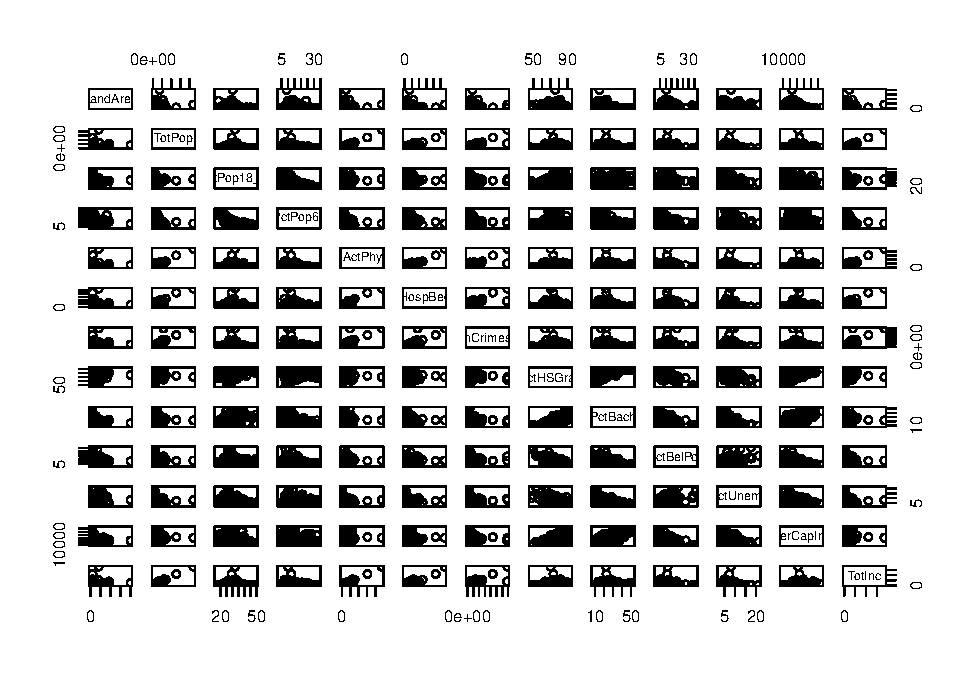
\includegraphics{Class_Exercises_ClassNotes_5_files/figure-latex/unnamed-chunk-39-1.pdf}
\newpage

\hypertarget{b-use-cor-to-make-the-correlation-matrix-of-the-data.-report-your-r-command.}{%
\paragraph{b) Use cor() to make the correlation matrix of the data.
Report your R
command.}\label{b-use-cor-to-make-the-correlation-matrix-of-the-data.-report-your-r-command.}}

\hfill\break
Code:

\begin{Shaded}
\begin{Highlighting}[]
\NormalTok{cor\_cdi }\OtherTok{\textless{}{-}} \FunctionTok{cor}\NormalTok{(}\FunctionTok{select}\NormalTok{(cdi, LandArea}\SpecialCharTok{:}\NormalTok{TotInc))}
\FunctionTok{head}\NormalTok{(cor\_cdi, }\DecValTok{3}\NormalTok{)}
\end{Highlighting}
\end{Shaded}

\begin{verbatim}
##                LandArea     TotPop PctPop18_34     PctPop65   nActPhys
## LandArea     1.00000000 0.17308335 -0.05487812  0.005770871 0.07807466
## TotPop       0.17308335 1.00000000  0.07837212 -0.029037393 0.94024859
## PctPop18_34 -0.05487812 0.07837212  1.00000000 -0.616309639 0.11969924
##              nHospBeds    nCrimes   PctHSGrad    PctBach  PctBelPov
## LandArea    0.07304727 0.12947537 -0.09859811 -0.1372377 0.17134335
## TotPop      0.92373836 0.88633185 -0.01742690  0.1468138 0.03801951
## PctPop18_34 0.07453191 0.08994063  0.25058429  0.4560970 0.03397551
##                 PctUnemp   PerCapInc     TotInc
## LandArea     0.199209277 -0.18771513 0.12707426
## TotPop       0.005351703  0.23561019 0.98674763
## PctPop18_34 -0.278527058 -0.03164843 0.07116151
\end{verbatim}

\begin{Shaded}
\begin{Highlighting}[]
\NormalTok{cdi\_nPhys }\OtherTok{\textless{}{-}} \FunctionTok{lm}\NormalTok{(nActPhys }\SpecialCharTok{\textasciitilde{}}\NormalTok{ TotPop }\SpecialCharTok{+}\NormalTok{ LandArea }\SpecialCharTok{+}\NormalTok{ TotInc, }\AttributeTok{data =}\NormalTok{ cdi)}
\FunctionTok{summary}\NormalTok{(cdi\_nPhys)}
\end{Highlighting}
\end{Shaded}

\begin{verbatim}
## 
## Call:
## lm(formula = nActPhys ~ TotPop + LandArea + TotInc, data = cdi)
## 
## Residuals:
##     Min      1Q  Median      3Q     Max 
## -1855.6  -215.2   -74.6    79.0  3689.0 
## 
## Coefficients:
##               Estimate Std. Error t value Pr(>|t|)    
## (Intercept) -1.332e+01  3.537e+01  -0.377 0.706719    
## TotPop       8.366e-04  2.867e-04   2.918 0.003701 ** 
## LandArea    -6.552e-02  1.821e-02  -3.597 0.000358 ***
## TotInc       9.413e-02  1.330e-02   7.078 5.89e-12 ***
## ---
## Signif. codes:  0 '***' 0.001 '**' 0.01 '*' 0.05 '.' 0.1 ' ' 1
## 
## Residual standard error: 560.4 on 436 degrees of freedom
## Multiple R-squared:  0.9026, Adjusted R-squared:  0.902 
## F-statistic:  1347 on 3 and 436 DF,  p-value: < 2.2e-16
\end{verbatim}

The Equation: Y = -1.332e+01 + 8.366e-04 * X1 - 6.552e-02 * X2 +
9.413e-02 * X3 \newpage

\hypertarget{d-obtain-the-predicted-number-of-active-physicians-for-a-county-with-a-total-population-of-400000-a-land-area-of-1000-square-miles-and-total-personal-income-of-8000-million-dollars-in-two-ways}{%
\paragraph{d) Obtain the predicted number of active physicians for a
county with a total population of 400,000, a land area of 1,000 square
miles, and total personal income of 8,000 million dollars in two
ways:}\label{d-obtain-the-predicted-number-of-active-physicians-for-a-county-with-a-total-population-of-400000-a-land-area-of-1000-square-miles-and-total-personal-income-of-8000-million-dollars-in-two-ways}}

\begin{enumerate}
\def\labelenumi{\arabic{enumi}.}
\tightlist
\item
  By plugging 400,000, 1,000, and 8,000 into the equation for X1, X2,
  and X3.
\item
  By using predict().
\end{enumerate}

\begin{Shaded}
\begin{Highlighting}[]
\SpecialCharTok{{-}}\FloatTok{13.32} \SpecialCharTok{+} \FloatTok{0.0008366} \SpecialCharTok{*} \DecValTok{400000} \SpecialCharTok{{-}} \FloatTok{0.06552} \SpecialCharTok{*} \DecValTok{1000} \SpecialCharTok{+} \FloatTok{0.09413} \SpecialCharTok{*} \DecValTok{8000}
\end{Highlighting}
\end{Shaded}

\begin{verbatim}
## [1] 1008.84
\end{verbatim}

\begin{Shaded}
\begin{Highlighting}[]
\NormalTok{newCdi }\OtherTok{\textless{}{-}} \FunctionTok{data.frame}\NormalTok{(}\AttributeTok{TotPop =} \DecValTok{400000}\NormalTok{, }
                     \AttributeTok{LandArea =} \DecValTok{1000}\NormalTok{,}
                     \AttributeTok{TotInc =} \DecValTok{8000}\NormalTok{)}
\FunctionTok{predict}\NormalTok{(cdi\_nPhys, }\AttributeTok{newdata =}\NormalTok{ newCdi)}
\end{Highlighting}
\end{Shaded}

\begin{verbatim}
##        1 
## 1008.864
\end{verbatim}

\hypertarget{e-how-much-does-number-of-active-physicians-increase-for-each-additional-1-person-increase-in-total-population-holding-land-area-and-total-personal-income-constant}{%
\paragraph{e) How much does number of active physicians increase for
each additional 1-person increase in total population (holding land area
and total personal income
constant)?}\label{e-how-much-does-number-of-active-physicians-increase-for-each-additional-1-person-increase-in-total-population-holding-land-area-and-total-personal-income-constant}}

\hfill\break
For each additional person, there is an increase of 0.0008366 active
physicians.

\hypertarget{f-how-much-does-number-of-active-physicians-increase-for-each-additional-1.0-million-dollars-in-totalpersonal-income-holding-land-area-and-total-population-constant}{%
\paragraph{f) How much does number of active physicians increase for
each additional 1.0 million dollars in totalpersonal income (holding
land area and total population
constant)?}\label{f-how-much-does-number-of-active-physicians-increase-for-each-additional-1.0-million-dollars-in-totalpersonal-income-holding-land-area-and-total-population-constant}}

\hfill\break
The increase in active physicians increases by 0.09413 for each
additional 1.0 million dollars in total personal income.

\hypertarget{exercise-11-do-the-following.}{%
\subsubsection{Exercise 11: Do the
following.}\label{exercise-11-do-the-following.}}

\hfill\break
Data frame:

\begin{Shaded}
\begin{Highlighting}[]
\NormalTok{cdi }\OtherTok{\textless{}{-}} \FunctionTok{mutate}\NormalTok{(cdi, }\AttributeTok{PopDens =}\NormalTok{ TotPop}\SpecialCharTok{/}\NormalTok{LandArea)}
\end{Highlighting}
\end{Shaded}

\newpage

\hypertarget{a-use-lm-to-fit-a-multiple-regression-model-with-number-of-active-physicians-as-the-response-y-and-population-density-x1-percent-of-population-65-or-older-x2-and-per-capita-income-x3-as-explanatory-variables.-then-use-summary-to-obtain-the-results.-report-the-equation-of-the-fitted-model.}{%
\paragraph{a) Use lm() to fit a multiple regression model with number of
active physicians as the response (Y ) and population density (X1),
percent of population 65 or older (X2), and per capita income (X3) as
explanatory variables. Then use summary() to obtain the results. Report
the equation of the fitted
model.}\label{a-use-lm-to-fit-a-multiple-regression-model-with-number-of-active-physicians-as-the-response-y-and-population-density-x1-percent-of-population-65-or-older-x2-and-per-capita-income-x3-as-explanatory-variables.-then-use-summary-to-obtain-the-results.-report-the-equation-of-the-fitted-model.}}

\hfill\break
Code:

\begin{Shaded}
\begin{Highlighting}[]
\NormalTok{cdi.reg }\OtherTok{\textless{}{-}} \FunctionTok{lm}\NormalTok{(nActPhys }\SpecialCharTok{\textasciitilde{}}\NormalTok{ PopDens }\SpecialCharTok{+}\NormalTok{ PctPop65 }\SpecialCharTok{+}\NormalTok{ PerCapInc, }\AttributeTok{data =}\NormalTok{ cdi)}
\FunctionTok{summary}\NormalTok{(cdi.reg)}
\end{Highlighting}
\end{Shaded}

\begin{verbatim}
## 
## Call:
## lm(formula = nActPhys ~ PopDens + PctPop65 + PerCapInc, data = cdi)
## 
## Residuals:
##     Min      1Q  Median      3Q     Max 
## -4998.0  -522.8  -293.8    64.2 22067.6 
## 
## Coefficients:
##               Estimate Std. Error t value Pr(>|t|)    
## (Intercept) -1.088e+03  4.240e+02  -2.566   0.0106 *  
## PopDens      2.873e-01  3.554e-02   8.083 6.27e-15 ***
## PctPop65    -7.964e+00  1.900e+01  -0.419   0.6753    
## PerCapInc    1.033e-01  1.921e-02   5.377 1.24e-07 ***
## ---
## Signif. codes:  0 '***' 0.001 '**' 0.01 '*' 0.05 '.' 0.1 ' ' 1
## 
## Residual standard error: 1589 on 436 degrees of freedom
## Multiple R-squared:  0.2173, Adjusted R-squared:  0.2119 
## F-statistic: 40.35 on 3 and 436 DF,  p-value: < 2.2e-16
\end{verbatim}

Equation: Y = -1.088e+03 + 2.873e-01 * x1 - 7.964e+00 * X2 + 1.033e-01 *
X3

\hypertarget{b-obtain-the-predicted-number-of-active-physicians-for-a-county-with-a-population-density-of-900-per-square-mile-15-percent-of-its-population-over-65-and-per-capita-income-of-20000-dollars-in-two-ways}{%
\paragraph{b) Obtain the predicted number of active physicians for a
county with a population density of 900 per square mile, 15 percent of
its population over 65, and per capita income of 20,000 dollars in two
ways:}\label{b-obtain-the-predicted-number-of-active-physicians-for-a-county-with-a-population-density-of-900-per-square-mile-15-percent-of-its-population-over-65-and-per-capita-income-of-20000-dollars-in-two-ways}}

\begin{enumerate}
\def\labelenumi{\arabic{enumi}.}
\tightlist
\item
  By plugging 900, 15, and 20,000 into the equation for X1, X2, and X3.
\item
  By using predict(). Report both sets of your R commands for obtaining
  the predicted number of active physicians.\\
  Code:
\end{enumerate}

\begin{Shaded}
\begin{Highlighting}[]
\SpecialCharTok{{-}}\FloatTok{1.088e+03} \SpecialCharTok{+} \FloatTok{2.873e{-}01} \SpecialCharTok{*} \DecValTok{900} \SpecialCharTok{{-}}\FloatTok{7.964e+00} \SpecialCharTok{*} \DecValTok{15} \SpecialCharTok{+} \FloatTok{1.033e{-}01} \SpecialCharTok{*} \DecValTok{20000}
\end{Highlighting}
\end{Shaded}

\begin{verbatim}
## [1] 1117.11
\end{verbatim}

\begin{Shaded}
\begin{Highlighting}[]
\NormalTok{newCdi\_PopDens }\OtherTok{\textless{}{-}} \FunctionTok{data.frame}\NormalTok{(}\AttributeTok{PopDens =} \DecValTok{900}\NormalTok{,}
                             \AttributeTok{PctPop65 =} \DecValTok{15}\NormalTok{,}
                             \AttributeTok{PerCapInc =} \DecValTok{20000}\NormalTok{)}
\FunctionTok{predict}\NormalTok{(cdi.reg, }\AttributeTok{newdata =}\NormalTok{ newCdi\_PopDens)}
\end{Highlighting}
\end{Shaded}

\begin{verbatim}
##        1 
## 1117.385
\end{verbatim}

\hypertarget{exercise-12-do-the-following.}{%
\subsubsection{Exercise 12: Do the
following.}\label{exercise-12-do-the-following.}}

\hfill\break
Data frame:

\begin{Shaded}
\begin{Highlighting}[]
\NormalTok{my.reg }\OtherTok{\textless{}{-}} \FunctionTok{lm}\NormalTok{(nActPhys }\SpecialCharTok{\textasciitilde{}}\NormalTok{ TotPop }\SpecialCharTok{+}\NormalTok{ LandArea }\SpecialCharTok{+}\NormalTok{ TotInc, }\AttributeTok{data =}\NormalTok{ cdi)}
\FunctionTok{summary}\NormalTok{(my.reg)}
\end{Highlighting}
\end{Shaded}

\begin{verbatim}
## 
## Call:
## lm(formula = nActPhys ~ TotPop + LandArea + TotInc, data = cdi)
## 
## Residuals:
##     Min      1Q  Median      3Q     Max 
## -1855.6  -215.2   -74.6    79.0  3689.0 
## 
## Coefficients:
##               Estimate Std. Error t value Pr(>|t|)    
## (Intercept) -1.332e+01  3.537e+01  -0.377 0.706719    
## TotPop       8.366e-04  2.867e-04   2.918 0.003701 ** 
## LandArea    -6.552e-02  1.821e-02  -3.597 0.000358 ***
## TotInc       9.413e-02  1.330e-02   7.078 5.89e-12 ***
## ---
## Signif. codes:  0 '***' 0.001 '**' 0.01 '*' 0.05 '.' 0.1 ' ' 1
## 
## Residual standard error: 560.4 on 436 degrees of freedom
## Multiple R-squared:  0.9026, Adjusted R-squared:  0.902 
## F-statistic:  1347 on 3 and 436 DF,  p-value: < 2.2e-16
\end{verbatim}

\begin{Shaded}
\begin{Highlighting}[]
\NormalTok{cdi }\OtherTok{\textless{}{-}} \FunctionTok{mutate}\NormalTok{(cdi, }\AttributeTok{PopDens =}\NormalTok{ TotPop }\SpecialCharTok{/}\NormalTok{ LandArea)}
\NormalTok{my.reg }\OtherTok{\textless{}{-}} \FunctionTok{lm}\NormalTok{(nActPhys }\SpecialCharTok{\textasciitilde{}}\NormalTok{ PopDens }\SpecialCharTok{+}\NormalTok{ PctPop65 }\SpecialCharTok{+}\NormalTok{ PerCapInc, }\AttributeTok{data =}\NormalTok{ cdi)}
\FunctionTok{summary}\NormalTok{(my.reg)}
\end{Highlighting}
\end{Shaded}

\begin{verbatim}
## 
## Call:
## lm(formula = nActPhys ~ PopDens + PctPop65 + PerCapInc, data = cdi)
## 
## Residuals:
##     Min      1Q  Median      3Q     Max 
## -4998.0  -522.8  -293.8    64.2 22067.6 
## 
## Coefficients:
##               Estimate Std. Error t value Pr(>|t|)    
## (Intercept) -1.088e+03  4.240e+02  -2.566   0.0106 *  
## PopDens      2.873e-01  3.554e-02   8.083 6.27e-15 ***
## PctPop65    -7.964e+00  1.900e+01  -0.419   0.6753    
## PerCapInc    1.033e-01  1.921e-02   5.377 1.24e-07 ***
## ---
## Signif. codes:  0 '***' 0.001 '**' 0.01 '*' 0.05 '.' 0.1 ' ' 1
## 
## Residual standard error: 1589 on 436 degrees of freedom
## Multiple R-squared:  0.2173, Adjusted R-squared:  0.2119 
## F-statistic: 40.35 on 3 and 436 DF,  p-value: < 2.2e-16
\end{verbatim}

\hypertarget{a-using-the-residual-standard-error-in-the-output-from-summary-which-model-fits-the-data-better-hint-a-smaller-residual-standard-error-indicates-a-better-fitting-model.}{%
\paragraph{a) Using the residual standard error in the output from
summary(), which model fits the data better? Hint: A smaller residual
standard error indicates a better fitting
model.}\label{a-using-the-residual-standard-error-in-the-output-from-summary-which-model-fits-the-data-better-hint-a-smaller-residual-standard-error-indicates-a-better-fitting-model.}}

\hfill\break
The better fitting model is the one containing the total population,
land area, and total income based on the residual standard error.

\hypertarget{b-using-the-r2-labeled-multiple-r-squared-in-the-output-from-summary-which-model-fits-the-data-better-hint-a-larger-r2-indicates-a-better-fitting-model.}{%
\paragraph{b) Using the R2 (labeled Multiple R-squared) in the output
from summary(), which model fits the data better? Hint: A larger R2
indicates a better fitting
model.}\label{b-using-the-r2-labeled-multiple-r-squared-in-the-output-from-summary-which-model-fits-the-data-better-hint-a-larger-r2-indicates-a-better-fitting-model.}}

\hfill\break
The first still indicates a better fitting model based on R2.

\hypertarget{c-based-on-your-answers-to-parts-a-and-b-which-model-would-you-expect-to-give-better-predictions-of-the-number-of-active-physicians-in-a-county}{%
\paragraph{c) Based on your answers to Parts a and b, which model would
you expect to give better predictions of the number of active physicians
in a
county?}\label{c-based-on-your-answers-to-parts-a-and-b-which-model-would-you-expect-to-give-better-predictions-of-the-number-of-active-physicians-in-a-county}}

\hfill\break
I would expect the first model to provide a better prediction based on
the two errors seen in parts \emph{a} and \emph{b}.

\begin{Shaded}
\begin{Highlighting}[]
\NormalTok{dues.file }\OtherTok{\textless{}{-}} \FunctionTok{file.choose}\NormalTok{()}

\NormalTok{dues }\OtherTok{\textless{}{-}} \FunctionTok{read.csv}\NormalTok{(dues.file, }\AttributeTok{header =} \ConstantTok{TRUE}\NormalTok{, }\AttributeTok{sep =} \StringTok{""}\NormalTok{, }\AttributeTok{stringsAsFactors =} \ConstantTok{FALSE}\NormalTok{)}

\FunctionTok{head}\NormalTok{(dues)}
\end{Highlighting}
\end{Shaded}

\begin{verbatim}
##   NotRenew DuesIncr
## 1        0       25
## 2        0       27
## 3        0       30
## 4        0       30
## 5        0       31
## 6        0       32
\end{verbatim}

\newpage

\hypertarget{section-9.7-exercises}{%
\subsection{Section 9.7 Exercises}\label{section-9.7-exercises}}

\hypertarget{exercise-13-do-the-following.}{%
\subsubsection{Exercise 13: Do the
following.}\label{exercise-13-do-the-following.}}

\begin{Shaded}
\begin{Highlighting}[]
\NormalTok{my.logreg }\OtherTok{\textless{}{-}}
  \FunctionTok{glm}\NormalTok{(NotRenew }\SpecialCharTok{\textasciitilde{}}\NormalTok{ DuesIncr, }\AttributeTok{family =} \StringTok{"binomial"}\NormalTok{, }\AttributeTok{data =}\NormalTok{ dues)}
\FunctionTok{summary}\NormalTok{(my.logreg)}
\end{Highlighting}
\end{Shaded}

\begin{verbatim}
## 
## Call:
## glm(formula = NotRenew ~ DuesIncr, family = "binomial", data = dues)
## 
## Deviance Residuals: 
##      Min        1Q    Median        3Q       Max  
## -2.12290  -0.37290   0.08522   0.47113   1.78651  
## 
## Coefficients:
##             Estimate Std. Error z value Pr(>|z|)   
## (Intercept) -15.4157     5.6780  -2.715  0.00663 **
## DuesIncr      0.3902     0.1421   2.745  0.00605 **
## ---
## Signif. codes:  0 '***' 0.001 '**' 0.01 '*' 0.05 '.' 0.1 ' ' 1
## 
## (Dispersion parameter for binomial family taken to be 1)
## 
##     Null deviance: 41.455  on 29  degrees of freedom
## Residual deviance: 20.083  on 28  degrees of freedom
## AIC: 24.083
## 
## Number of Fisher Scoring iterations: 6
\end{verbatim}

\hypertarget{a-obtain-the-estimated-probability-that-a-person-wont-renew-their-membership-if-the-dues-increase-is-45-dollars-in-two-ways}{%
\paragraph{a) Obtain the (estimated) probability that a person won't
renew their membership if the dues increase is 45 dollars in two
ways:}\label{a-obtain-the-estimated-probability-that-a-person-wont-renew-their-membership-if-the-dues-increase-is-45-dollars-in-two-ways}}

\begin{enumerate}
\def\labelenumi{\arabic{enumi}.}
\tightlist
\item
  By plugging 45 into the equation for X.
\item
  By using predict().\\
  Code:
\end{enumerate}

\begin{Shaded}
\begin{Highlighting}[]
\FunctionTok{exp}\NormalTok{(}\SpecialCharTok{{-}}\FloatTok{15.42} \SpecialCharTok{+} \FloatTok{0.39} \SpecialCharTok{*} \DecValTok{45}\NormalTok{)}\SpecialCharTok{/}\NormalTok{(}\DecValTok{1} \SpecialCharTok{+} \FunctionTok{exp}\NormalTok{(}\SpecialCharTok{{-}}\FloatTok{15.42} \SpecialCharTok{+} \FloatTok{0.39} \SpecialCharTok{*} \DecValTok{45}\NormalTok{))}
\end{Highlighting}
\end{Shaded}

\begin{verbatim}
## [1] 0.893785
\end{verbatim}

\begin{Shaded}
\begin{Highlighting}[]
\NormalTok{newDues }\OtherTok{\textless{}{-}} \FunctionTok{data.frame}\NormalTok{(}\AttributeTok{DuesIncr =} \DecValTok{45}\NormalTok{)}
\FunctionTok{predict}\NormalTok{(my.logreg, newDues, }\AttributeTok{type =} \StringTok{"response"}\NormalTok{)}
\end{Highlighting}
\end{Shaded}

\begin{verbatim}
##        1 
## 0.894954
\end{verbatim}

\hypertarget{b-now-obtain-the-estimated-probability-that-a-person-wont-renew-their-membership-if-the-dues-increase-is-only-35-dollars-dollars-in-two-ways}{%
\paragraph{b) Now obtain the (estimated) probability that a person won't
renew their membership if the dues increase is only 35 dollars dollars
in two
ways:}\label{b-now-obtain-the-estimated-probability-that-a-person-wont-renew-their-membership-if-the-dues-increase-is-only-35-dollars-dollars-in-two-ways}}

\begin{enumerate}
\def\labelenumi{\arabic{enumi}.}
\tightlist
\item
  By plugging 35 into the equation for X.
\item
  By using predict(). Report both sets of your R commands for obtaining
  the (estimated) probability of not renewing.\\
  Code:
\end{enumerate}

\begin{Shaded}
\begin{Highlighting}[]
\FunctionTok{exp}\NormalTok{(}\SpecialCharTok{{-}}\FloatTok{15.42} \SpecialCharTok{+} \FloatTok{0.39} \SpecialCharTok{*} \DecValTok{35}\NormalTok{)}\SpecialCharTok{/}\NormalTok{(}\DecValTok{1} \SpecialCharTok{+} \FunctionTok{exp}\NormalTok{(}\SpecialCharTok{{-}}\FloatTok{15.42} \SpecialCharTok{+} \FloatTok{0.39} \SpecialCharTok{*} \DecValTok{35}\NormalTok{))}
\end{Highlighting}
\end{Shaded}

\begin{verbatim}
## [1] 0.1455423
\end{verbatim}

\begin{Shaded}
\begin{Highlighting}[]
\NormalTok{newDues }\OtherTok{\textless{}{-}} \FunctionTok{data.frame}\NormalTok{(}\AttributeTok{DuesIncr =} \DecValTok{35}\NormalTok{)}
\FunctionTok{predict}\NormalTok{(my.logreg, newDues, }\AttributeTok{type =} \StringTok{"response"}\NormalTok{)}
\end{Highlighting}
\end{Shaded}

\begin{verbatim}
##         1 
## 0.1468632
\end{verbatim}

\newpage

i \#\# Section 9.8 Exercises

\hypertarget{exercise-14-do-the-following.}{%
\subsubsection{Exercise 14: Do the
following.}\label{exercise-14-do-the-following.}}

\hfill\break
Data:

\begin{Shaded}
\begin{Highlighting}[]
\NormalTok{Ln }\OtherTok{\textless{}{-}} \FunctionTok{c}\NormalTok{(}\FloatTok{85.7}\NormalTok{, }\FloatTok{64.5}\NormalTok{, }\FloatTok{84.1}\NormalTok{, }\FloatTok{82.5}\NormalTok{, }\FloatTok{78.0}\NormalTok{, }\FloatTok{81.3}\NormalTok{, }\FloatTok{71.0}\NormalTok{, }\FloatTok{86.7}\NormalTok{, }\FloatTok{78.7}\NormalTok{)}
\NormalTok{Wt }\OtherTok{\textless{}{-}}
  \FunctionTok{c}\NormalTok{(}\FloatTok{331.9}\NormalTok{, }\FloatTok{121.5}\NormalTok{, }\FloatTok{382.2}\NormalTok{, }\FloatTok{287.3}\NormalTok{, }\FloatTok{224.3}\NormalTok{, }\FloatTok{245.2}\NormalTok{, }\FloatTok{208.2}\NormalTok{, }\FloatTok{393.4}\NormalTok{, }\FloatTok{228.3}\NormalTok{)}
\NormalTok{snakes }\OtherTok{\textless{}{-}} \FunctionTok{data.frame}\NormalTok{(}\AttributeTok{Length =}\NormalTok{ Ln, }\AttributeTok{Weight =}\NormalTok{ Wt)}

\NormalTok{g }\OtherTok{\textless{}{-}} \FunctionTok{ggplot}\NormalTok{(Snakes, }\FunctionTok{aes}\NormalTok{(}\AttributeTok{x =}\NormalTok{ Ln, }\AttributeTok{y =}\NormalTok{ Wt)) }\SpecialCharTok{+} \FunctionTok{geom\_point}\NormalTok{()}
\CommentTok{\# Eighth degree polynomial model (Model 8):}
\NormalTok{g }\SpecialCharTok{+} \FunctionTok{stat\_smooth}\NormalTok{(}\AttributeTok{method =} \StringTok{"lm"}\NormalTok{,}
                \AttributeTok{formula =}\NormalTok{ y }\SpecialCharTok{\textasciitilde{}} \FunctionTok{poly}\NormalTok{(x, }\DecValTok{8}\NormalTok{),}
                \AttributeTok{se =}\NormalTok{ F) }\SpecialCharTok{+}
  \FunctionTok{ggtitle}\NormalTok{(}\AttributeTok{label =} \StringTok{"Model 8"}\NormalTok{)}
\end{Highlighting}
\end{Shaded}

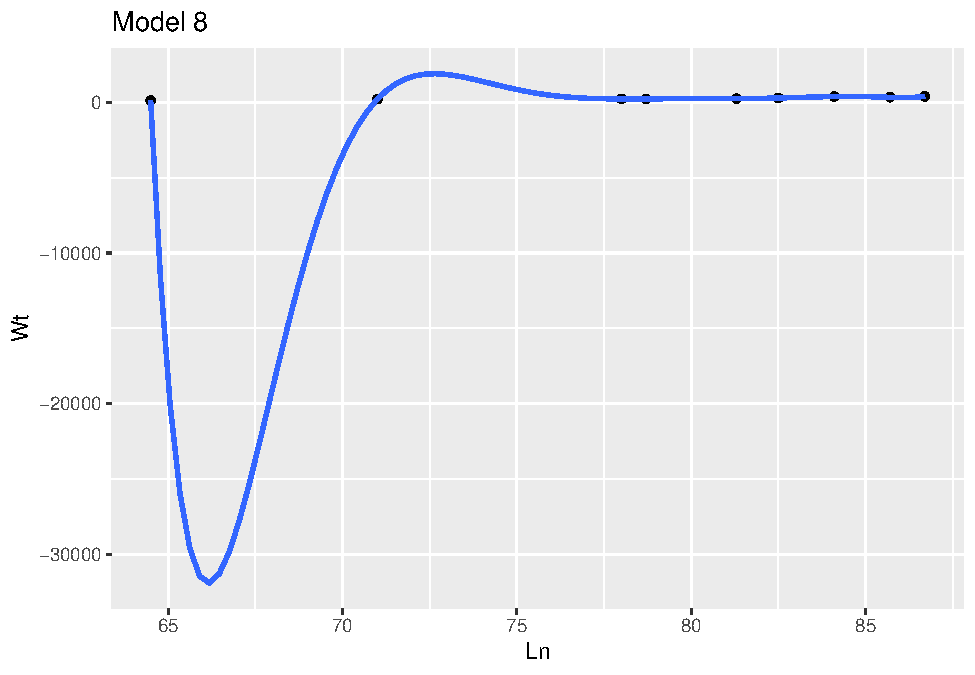
\includegraphics{Class_Exercises_ClassNotes_5_files/figure-latex/unnamed-chunk-51-1.pdf}
\newpage

\begin{Shaded}
\begin{Highlighting}[]
\NormalTok{g }\SpecialCharTok{+} \FunctionTok{stat\_smooth}\NormalTok{(}\AttributeTok{method =} \StringTok{"lm"}\NormalTok{, }\AttributeTok{formula =}\NormalTok{ y }\SpecialCharTok{\textasciitilde{}}\NormalTok{ x, }\AttributeTok{se =}\NormalTok{ F) }\SpecialCharTok{+}
  \FunctionTok{ggtitle}\NormalTok{(}\AttributeTok{label =} \StringTok{"Linear Model"}\NormalTok{)}
\end{Highlighting}
\end{Shaded}

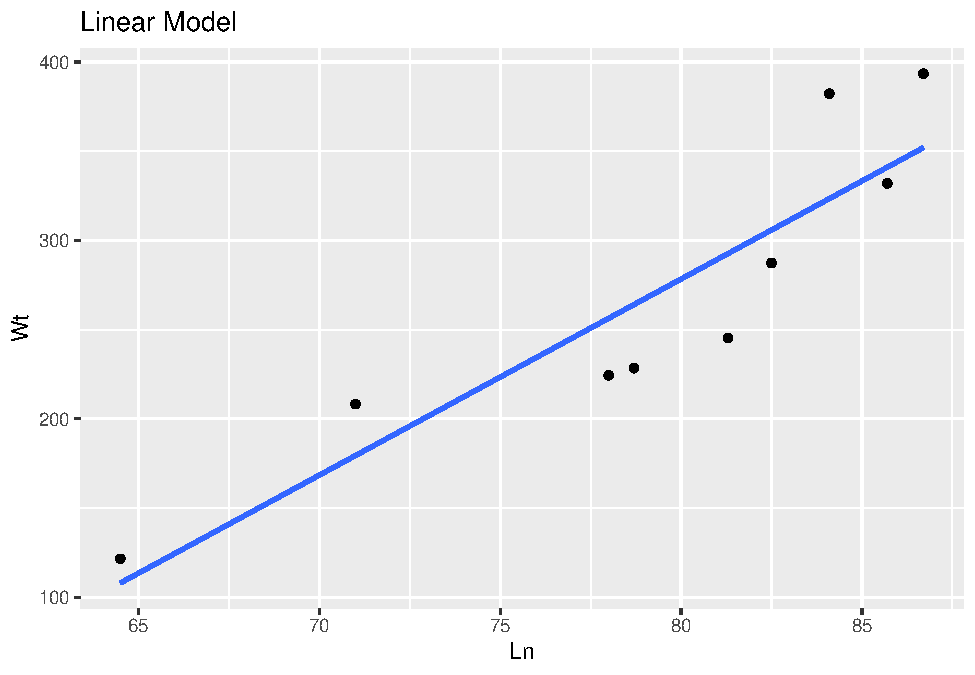
\includegraphics{Class_Exercises_ClassNotes_5_files/figure-latex/unnamed-chunk-52-1.pdf}
\newpage

\begin{Shaded}
\begin{Highlighting}[]
\CommentTok{\# Models with five new snakes}
\NormalTok{newSnakes }\OtherTok{\textless{}{-}} \FunctionTok{data.frame}\NormalTok{(}\AttributeTok{Ln =} \FunctionTok{c}\NormalTok{(}\DecValTok{67}\NormalTok{, }\DecValTok{72}\NormalTok{, }\DecValTok{77}\NormalTok{, }\DecValTok{81}\NormalTok{, }\DecValTok{86}\NormalTok{),}
                        \AttributeTok{Wt =} \FunctionTok{c}\NormalTok{(}\FloatTok{127.9}\NormalTok{, }\FloatTok{153.7}\NormalTok{, }\FloatTok{204.7}\NormalTok{, }\FloatTok{300.6}\NormalTok{,   }\FloatTok{291.4}\NormalTok{))}

\NormalTok{g\_new }\OtherTok{\textless{}{-}} \FunctionTok{ggplot}\NormalTok{(Snakes, }\FunctionTok{aes}\NormalTok{(}\AttributeTok{x =}\NormalTok{ Ln, }\AttributeTok{y =}\NormalTok{ Wt)) }\SpecialCharTok{+}
  \FunctionTok{geom\_point}\NormalTok{(}\AttributeTok{alpha =} \FloatTok{0.05}\NormalTok{)}

\NormalTok{g\_new }\SpecialCharTok{+} \FunctionTok{stat\_smooth}\NormalTok{(}\AttributeTok{method =} \StringTok{"lm"}\NormalTok{,}
                    \AttributeTok{formula =}\NormalTok{ y }\SpecialCharTok{\textasciitilde{}} \FunctionTok{poly}\NormalTok{(x, }\DecValTok{8}\NormalTok{),}
                    \AttributeTok{se =}\NormalTok{ F) }\SpecialCharTok{+}
  \FunctionTok{ggtitle}\NormalTok{(}\AttributeTok{label =} \StringTok{"Model 8 with New Snakes"}\NormalTok{) }\SpecialCharTok{+}
  \FunctionTok{geom\_point}\NormalTok{(}\AttributeTok{data =}\NormalTok{ newSnakes)}
\end{Highlighting}
\end{Shaded}

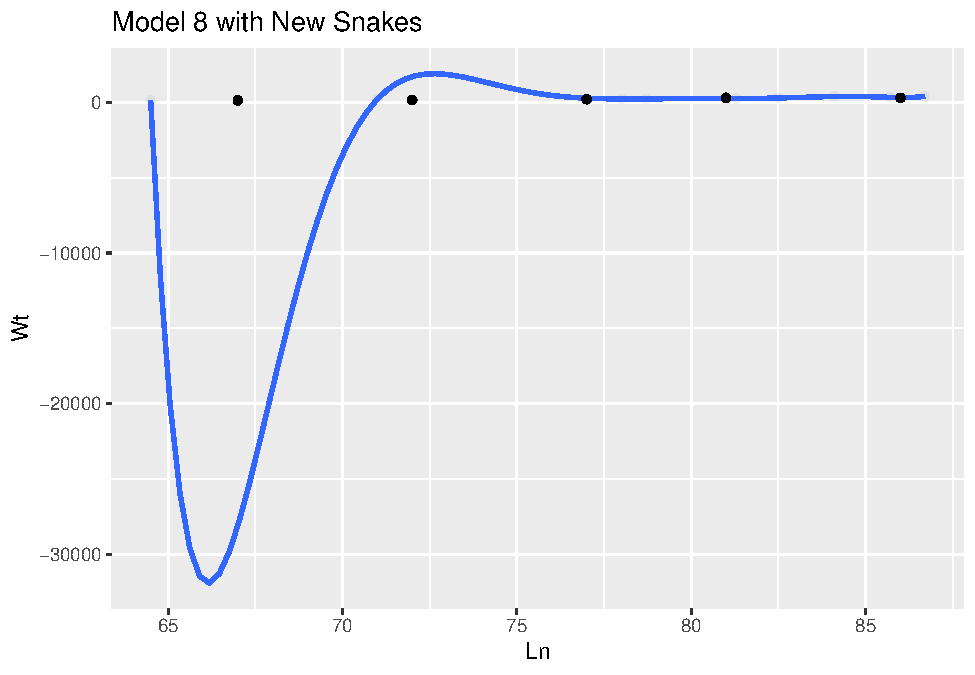
\includegraphics{Class_Exercises_ClassNotes_5_files/figure-latex/unnamed-chunk-53-1.pdf}
\newpage

\begin{Shaded}
\begin{Highlighting}[]
\NormalTok{g\_new }\SpecialCharTok{+} \FunctionTok{stat\_smooth}\NormalTok{(}\AttributeTok{method =} \StringTok{"lm"}\NormalTok{,}
                    \AttributeTok{formula =}\NormalTok{ y }\SpecialCharTok{\textasciitilde{}}\NormalTok{ x,}
                    \AttributeTok{se =}\NormalTok{ F) }\SpecialCharTok{+}
  \FunctionTok{ggtitle}\NormalTok{(}\AttributeTok{label =} \StringTok{"Linear Model with New Snakes"}\NormalTok{) }\SpecialCharTok{+}
  \FunctionTok{geom\_point}\NormalTok{(}\AttributeTok{data =}\NormalTok{ newSnakes)}
\end{Highlighting}
\end{Shaded}

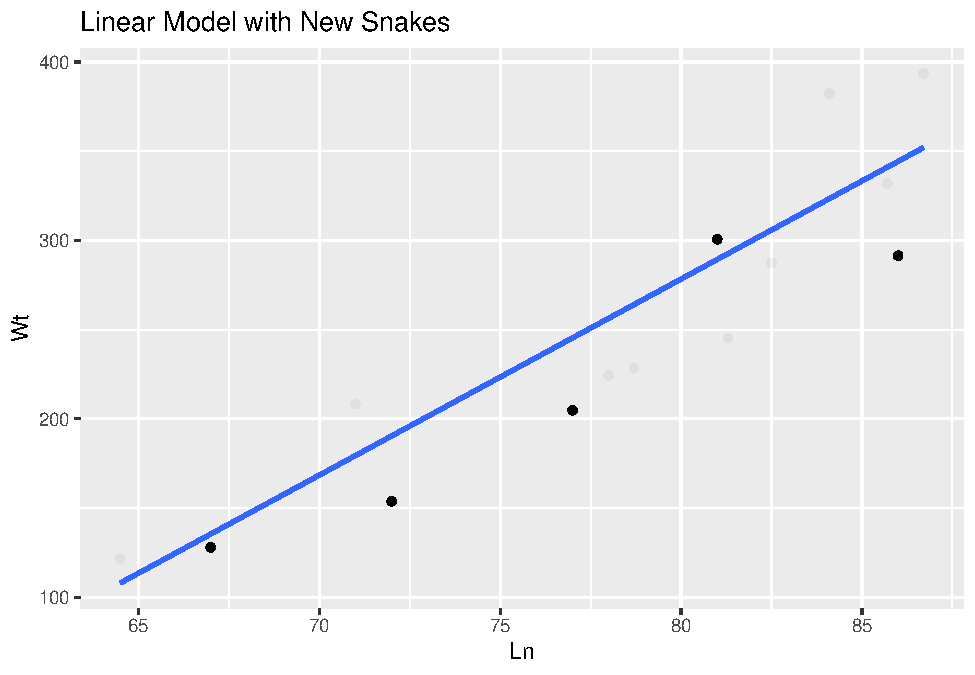
\includegraphics{Class_Exercises_ClassNotes_5_files/figure-latex/unnamed-chunk-54-1.pdf}

\hypertarget{a-how-well-does-the-fitted-model-predict-the-weights-of-the-original-nine-snakes}{%
\paragraph{a) How well does the fitted model predict the weights of the
original nine
snakes?}\label{a-how-well-does-the-fitted-model-predict-the-weights-of-the-original-nine-snakes}}

\hfill\break
The model 8 graph seems to fit the points better than the linear model.

\hypertarget{b-how-well-do-you-think-the-fitted-model-would-predict-the-weights-of-five-new-snakes}{%
\paragraph{b) How well do you think the fitted model would predict the
weights of five new
snakes?}\label{b-how-well-do-you-think-the-fitted-model-would-predict-the-weights-of-five-new-snakes}}

\hfill\break
The model 8 had a huge amount of error in one of the points for a sample
of new snakes. Overall, the new snakes fit better with the linear model
even though the linear model has the appearance of more error for more
of the points.

\end{document}
